\documentclass[german]{spicker}

%\addbibresource{num1.bib}

\title{Numerik 1}
\author{Patrick Gustav Blaneck}
\makeindex[intoc]
\makeindex[intoc, name=Beispiele,title=Beispiele]

\begin{document}
\maketitle
\tableofcontents
\newpage

\section{Einleitung}

\begin{defi}{Numerik}
    Lloyd Trefethen 1992:
    \begin{displayquote}
        Numerical analysis is the study of algorithms for the problems of continuous mathematics.
    \end{displayquote}

    \enquote{continuous mathematics} heißt, dass reelle oder komplexe Zahlen beteiligt sind, in Abgrenzung zur diskreten Mathematik.
    Dies umfasst die Analysis und Teile der linearen Algebra.

    Die \emph{Numerik} beschäftigt sich mit der Entwicklung von (effizienten) Berechnungsmethoden, da viele mathematische Objekte zwar wohldefiniert sind, aber nicht endlich berechenbar.
\end{defi}

\begin{example}{Auswertung der Exponentialfunktion}
    Zu berechnen sei $e^{\frac{1}{2}}$, wie Exponentialfunktion bekanntermaßen wie folgt definiert ist:
    \[
        e^x = \sum_{k=0}^\infty \frac{x^k}{k!}
    \]

    Die unendliche Summe ist nicht direkt berechenbar, daher wird ein Ersatzproblem gelöst:
    \[
        e^x \approx \sum_{k=0}^n \frac{x^k}{k!}
    \]
    Dabei ist $n$ ein neuer freier Parameter.
    Es gilt:
    \begin{itemize}
        \item kleines $n$ $\implies$ eventuell zu viel vernachlässigt, Wert ungenau approximiert.
        \item großes $n$ $\implies$ Berechnung aufwändig, Gewinn an Genauigkeit potentiell gering.
    \end{itemize}

    Ein weiteres Problem kann durch eine nicht-exakte Arithmetik aufkommen.
    Seien die beiden Summationsreihenfolgen $s_1(x)$ und $s_2(x)$ gegeben:
    \[
        s_1(x) = 1 + x + \frac{x^2}{2} + \ldots + \frac{x^n}{n!}
    \]
    \[
        s_2(x) = \frac{x^n}{n!} + \ldots + \frac{x^2}{2} + x + 1
    \]

    Bei einer Floating-Point-Rechnung mit 3 Stellen Genauigkeit gilt:
    \begin{center}
        \begin{tabular}{|C||C|C|C|C|C|}
            \hline
            n        & 1   & 2    & 3    & 4    & 5    \\
            \hline
            \hline
            s_1(0.5) & 1.5 & 1.62 & 1.64 & 1.64 & 1.64 \\
            \hline
            s_2(0.5) & 1.5 & 1.62 & 1.65 & 1.65 & 1.65 \\
            \hline
        \end{tabular}
    \end{center}

    Die Summationsreihenfolge beeinflusst also das Ergebnis.

    Ein Abbruch bei $n=4$ ist für $x = \nicefrac{1}{2}$ angemessen.
\end{example}


\begin{example}{Rechteckregel und Trapezregel}
    Zu approximieren sei die Funktion
    \[
        f(x) = \int_{0}^{1} \frac{1}{1+x^2} \diff x
    \]

    \emph{Rechteckregel} und \emph{Trapezregel} approximieren diese Funktion wie folgt:

    % Rechteckregel
    \begin{tikzpicture}
        \begin{axis}[
                axis lines = left,
                %xlabel = $x$,
                %ylabel = $f(x)$,
                xmin = 0,
                xmax = 1.05,
                ymin = 0,
                ymax = 1.05,
            ]

            \addplot[name path=f,domain = 0:1.05,samples = 100] { 1/(1+x^2) };

            \addplot[dashed] coordinates{(1,0) (1,1)};

            \path[name path=axis] (axis cs:0,0) -- (axis cs:1,0);
            \path[name path=approx] (axis cs:0,1) -- (axis cs:1,1);

            \addplot[fill=red,fill opacity=0.1] fill between[of=approx and axis,soft clip={domain=0:1}];
        \end{axis}
    \end{tikzpicture}
    % Trapezregel
    \begin{tikzpicture}
        \begin{axis}[
                axis lines = left,
                %xlabel = $x$,
                %ylabel = $f(x)$,
                xmin = 0,
                xmax = 1.05,
                ymin = 0,
                ymax = 1.05,
            ]

            \addplot[name path=f,domain = 0:1.05,samples = 100] { 1/(1+x^2) };

            \addplot[dashed] coordinates{(1,0) (1,1)};

            \path[name path=axis] (axis cs:0,0) -- (axis cs:1,0);
            \path[name path=approx] (axis cs:0,1) -- (axis cs:1,0.5);

            \addplot[fill=blue,fill opacity=0.1] fill between[of=approx and axis,soft clip={domain=0:1}];
        \end{axis}
    \end{tikzpicture}

    TO DO
\end{example}

\begin{defi}{Numerische Simulation}
    \emph{Numerische Simulation} beschreibt die Verhaltensvorhersage eines physikalischen Systems durch mathematische Modelle und numerische Verfahren.

    Numerische Simulationen sind z.B. anwendbar in physikalischen Systemen (beliebige Bauteile) und daher sehr wichtig für die Produktentwicklung in der Industrie.

    Das Vorgehen ist wie folgt:
    \begin{itemize}
        \item virtueller Prototyp: vollständige Analyse durch numerische Simulation
        \item davon ausgehend: endgültige Auslegung der Konstruktion
        \item am Ende: Validierung durch einen realen Prototypen
    \end{itemize}

    In der Regel spart numerische Simulation Geld und Zeit.
\end{defi}
\section{Lineare Gleichungssysteme - Direkte Löser I}
\section{Fehlerbetrachtung}

\begin{defi}{Gut gestelltes Problem}
    Praktisch alle Aufgabenstellungen der numerischen Mathematik lassen sich als (eventuell sehr kompliziertes) Nullstellenproblem schreiben:
    \begin{itemize}
        \item gegeben ist eine Funktion $g$ und Eingabedaten $x$
        \item suche $y$ mit $g(x, y) = 0$
    \end{itemize}

    Folgende Eigenschaften sollte ein solches Problem sinnvollerweise erfüllen:
    \begin{itemize}
        \item \emph{Existenz}: es sollte Lösungen geben
        \item \emph{Eindeutigkeit}: zu jedem $x$ sollte es genau ein $y$ geben
        \item \emph{Stetige Abhängigkeit}:\footnote{Stetige Abhängigkeit garantiert, dass (hinreichend) kleine Störungen der Eingabedaten nur kleine Veränderungen der Ergebnisse verursachen.} der Lösung $y$ von den Eingabedaten $x$, d. h.
              \[
                  x' \to x \quad \implies \quad y' = f(x') \to f(x) = y
              \]
    \end{itemize}

    Gilt für das Problem $g(x, y) = 0$ Existenz, Eindeutigkeit und stetige Abhängigkeit, so nennt man das Problem \emph{gut gestellt} (\enquote{well posed}), ansonsten \emph{schlecht gestellt} (\enquote{ill posed}).

    Müssen schlecht gestellte Probleme behandelt werden, so approximiert man sie in der Regel durch gut gestellte Ersatzprobleme (Regularisierung), wobei die Approximationseigenschaften genau kontrolliert werden müssen.
\end{defi}

\begin{example}{Gut gestelltes Problem}

    \begin{itemize}
        \item Ein lineares Gleichungssystem $Ax = b$ ist äquivalent zu:
              \[
                  g(x, y) = 0, \quad x = (A, b), \quad g(x, y) = Ay - b
              \]

              Wir erhalten:
              \[
                  y = f(x) = A^{-1} b, \quad x = (A, b), \quad \det(A) \neq 0
              \]
        \item Die größere der beiden Nullstellen von $t^2 + 2pt - q = 0$, $p, q > 0$ ist gegeben durch:
              \[
                  t_2 = -p + \sqrt{p^2 + q}
              \]
              d. h. das Nullstellenproblem ist äquivalent zu:
              \[
                  g(x, y) = 0, \quad x = (p, q), \quad g(x, y) = y - (-p + \sqrt{p^2 + q})
              \]

              Wir erhalten:
              \[
                  y = f(x) = -p + \sqrt{p^2 + q}, \quad x = (p, q)^T, \quad p, q > 0
              \]
    \end{itemize}

    Beide Funktionen sind stetig, so dass beide Probleme gut gestellt sind.
\end{example}

\subsection{Fehlergrößen}

\begin{defi}{Fehler}
    Sei ein gut gestelltes Problem
    \[
        y = f(x), \quad f: X \to Y
    \]
    gegeben mit:
    \begin{itemize}
        \item $x$ bekannt
        \item $X$ und $Y$ sind Vektorräume mit Normen $\| \cdot \|_X$ bzw. $\| \cdot \|_Y$
    \end{itemize}

    Zur numerischen Behandlung wird $f$ durch ein (diskretes, endliches) Problem $\hat{f}$ ersetzt, das anschließend in Floating-Point-Arithmetik als $\tilde{f}$ implementiert wird.

    Wir kennen also:
    \begin{itemize}
        \item $f(x) = y$:
              \begin{itemize}
                  \item $x$ sind \emph{exakte Eingabedaten}
                  \item $f$ ist ein \emph{gut gestelltes Problem}
                  \item $y$ ist die \emph{exakte Lösung}
              \end{itemize}
        \item $\hat{f}(x) = \hat{y}$:
              \begin{itemize}
                  \item $x$ sind exakte Eingabedaten
                  \item $\hat{f}$ ist das \emph{Ersatzproblem}
                  \item $\hat{y}$ ist die \emph{exakte Lösung des Ersatzproblems}
              \end{itemize}
        \item $\tilde{f}(\tilde{x}) = \tilde{y}$:
              \begin{itemize}
                  \item $\tilde{x}$ sind Eingabedaten in \emph{Floating-Point-Darstellung}
                  \item $\tilde{f}$ ist die \emph{Floating-Point-Implementierung des Ersatzproblems}
                  \item $\tilde{y}$ ist das \emph{Ergebnis des in Floating-Point-Arithmetik durchgeführten Ersatzproblems}
              \end{itemize}
    \end{itemize}

    Die Qualität eines Approximationsverfahrens wird dadurch bestimmt, wie weit $\tilde{y}$ von $y$ abweicht.
    Um diese Abweichung quantitativ zu fassen, werden die folgenden Fehlergrößen definiert:
    \begin{itemize}
        \item \emph{Fehler}:
              \[
                  e := \tilde{y} - y
              \]
        \item \emph{absoluter Fehler}:
              \[
                  e_a := \| \tilde{y} - y \|_Y
              \]
        \item \emph{relativer Fehler}:
              \[
                  e_r := \frac{\| \tilde{y} - y \|_Y}{\| y \|_Y}, \quad \| y \|_Y \neq 0
              \]
    \end{itemize}
\end{defi}

\begin{defi}{Gemischtes Fehlerkriterium}
    In numerischen Verfahren versucht man den Fehler zu kontrollieren und dabei (wenn möglich) unter eine
    vom Benutzer vorgegebene Schranke $\epsilon$ zu drücken.

    Der relative Fehler ist eigentlich aussagekräftiger, kann aber bei kleinen Absolutwerten von $y$ eine unnötig hohe Genauigkeit erzwingen.
    Deshalb benutzt man in der Praxis häufig ein Kriterium, das beide Fehlerarten kombiniert.

    Seien $\epsilon_a$ und $\epsilon_r$ gegebene Schranken für den absoluten bzw. relativen Fehler.

    Beim \emph{gemischten Fehlerkriterium} versucht man eine Approximation $\tilde{y}$ von $y$ zu finden, mit
    \[
        \| \tilde{y} - y \|_Y \leq \epsilon_a + \| y \|_Y \epsilon_r
    \]

    Es gilt:
    \begin{itemize}
        \item Ist der exakte Absolutwert $\| y \|_Y$ sehr klein, dann dominiert $\epsilon_a$ und
              \[
                  e_a = \| \tilde{y} - y \|_Y \lesssim \epsilon_a
              \]
        \item Ist der exakte Absolutwert $\| y \|_Y$ sehr groß, dann dominiert $\|y \|_Y \epsilon_r$ und
              \[
                  \| \tilde{y} - y \|_Y \lesssim \|y \|_Y \epsilon_r \quad \iff \quad e_r = \frac{\| \tilde{y} - y \|_Y}{\| y \|_Y} \lesssim \epsilon_r
              \]
    \end{itemize}
\end{defi}

\subsection{Fehlerquellen}

\begin{defi}{Eingabefehler}
    Wegen der Umwandlung der Eingabedaten $x$ in Floating-Point-Darstellung $\tilde{x}$ tritt der \emph{Eingabefehler} immer auf und wird deshalb auch als \emph{unvermeidbarer Fehler} bezeichnet:
    \[
        f(\tilde{x}) - f(x)
    \]

    Die Größe dieses Fehleranteils hängt davon ab, wie empfindlich das Originalproblem $f$ auf Störungen in den Eingabedaten reagiert.
\end{defi}

\begin{defi}{Verfahrensfehler}
    Beim \emph{Verfahrensfehler} wird das in exakter Arithmetik gerechnete Ersatzproblem $\hat{f}$ mit dem Originalproblem $f$ für den selben Input $\tilde{x}$ verglichen:
    \[
        \hat{f}(\tilde{x}) - f(\tilde{x})
    \]

    Die Größe dieses Fehleranteils hängt von der Qualität des Ersatzproblems ab.
\end{defi}

\begin{defi}{Akkumulierter Rundungsfehler}
    Das Ersatzproblem $\hat{f}$ besteht aus einer endlichen Anzahl von Elementaroperationen (Additionen, Multiplikationen etc.), die bei der Floating-Point-Implementierung $\tilde{f}$ durch ihre Floating-Point-Äquivalente ersetzt werden.

    Jede Floating-Point-Operation erzeugt in der Regel Rundungsfehler, die sich akkumulieren.

    Die Größe dieses Fehleranteils hängt davon ab, wie robust das Ersatzproblem auf eine Floating-Point-Implementierung reagiert:
    \[
        \tilde{f}(\tilde{x}) - \hat{f}(\tilde{x})
    \]
\end{defi}

\begin{defi}{Fließkommazahl}
    Eine \emph{Fließkommazahl} zur Basis $b$ hat die Darstellung
    \[
        v \cdot m \cdot b^e
    \]
    Dabei ist:
    \begin{itemize}
        \item $b \in \N$ die \emph{Basis}
        \item $v = \pm 1$ das \emph{Vorzeichen}
        \item $m$ die \emph{Mantisse}, ein $b$-adischer Bruch
              \[
                  m = m_{-k} \ldots m_{-1}m_0 . m_1 \ldots m_l \quad \iff \quad m = \sum_{i = -k}^{l} m_i \cdot b^{-i}
              \]
              mit Ziffern $m_i \in \{ 0, 1, \ldots, b-1 \}$ und Stellenzahl $k + l + 1$
        \item $e \in \Z$ der \emph{Exponent}
    \end{itemize}

    In dieser Form sind Fließkommadarstellungen einer Zahl nicht eindeutig, denn durch Änderung des Exponenten erhält man z. B.
    \begin{itemize}
        \item $\num{-43210000}$
        \item $-43.21 \cdot 10^6$
        \item $-4.321 \cdot 10^7$
    \end{itemize}

    Die \emph{normalisierte Darstellung}
    \[
        m = \pm (m_0 . m_1 \ldots m_l) \cdot b^e \quad \iff \quad m = \pm \left( \sum_{i = 0}^{l} m_i b^{-i} \right) \cdot b^e, \quad m_0 \neq 0
    \]
    ist für Zahlen $\neq 0$ eindeutig.
\end{defi}

\begin{defi}{Maschinengenauigkeit}
    Jede reelle Zahl $x \in \R$ kann als normalisierte Fließkommazahl zur Basis $b$ mit unendlich langer Mantisse dargestellt werden.

    Durch Runden erzeugt man aus $x$ eine Fließkommazahl $\tilde{x}$ mit Stellenzahl $l + 1$.
    Dazu wird in der Regel dasjenige $\tilde{x}$ ausgewählt, das $x$ am nächsten liegt (\emph{nearest Rundung}.)

    Betrachten wir normierte Fließkommazahlen zur Basis $b$ mit Mantissenlänge $l$, so bezeichnet
    \[
        \epsilon_M := \frac{1}{2} b^{-l}
    \]
    die \emph{Maschinengenauigkeit}.

    Es gilt:
    \begin{itemize}
        \item $\epsilon_M$ ist der maximale relative Fehler, der bei der Umwandlung einer rellen Zahl (bei nearest Rundung) entstehen kann.
        \item $\epsilon_M$ hängt nur von der Basis und der Mantissenlänge, nicht aber vom Exponenten ab.
    \end{itemize}
\end{defi}

\begin{defi}{Kondition}
    Sei $f: X \to Y$.
    Die kleinsten Konstanten $\varkappa_a$, $\varkappa_r$ mit
    \[
        \| f(x') - f(x) \|_Y \leq \varkappa_a \| x' - x \|_X
    \]
    \[
        \frac{\| f(x') - f(x) \|_Y}{\| f(x) \|_Y} \leq \varkappa_r \frac{\| x' - x \|_X}{\| x \|_X}
    \]
    und
    \[
        \| x' - x \|_X \leq \delta
    \]
    heißen \emph{absolute Kondition} bzw. \emph{relative Kondition} von $f$ in $x$ und hängen von den benutzten Normen, $x$ und $\delta$ ab.

    Die Konditionszahlen beschreiben, wie stark $f$ Störungen in $x$ schlimmstenfalls verstärkt.

    Kleine Konditionszahlen deuten auf ein gut konditioniertes, große auf ein schlecht konditioniertes Problem hin.

    Werden die Störungen in $x$ durch die Umwandlung in ein Floating-Point-Format verursacht, d.h. $x' =  \tilde{x}$, so gilt:
    \[
        e_r(x) = \frac{\| \tilde{x} - x \|_X}{\| x \|_X} \leq \epsilon_M
    \]
    bzw.
    \[
        e_r(y) = \frac{\| \tilde{y} - y \|_Y}{\| y \|_Y} \leq \varkappa_r \frac{\| \tilde{x} - x \|_X}{\| x \|_X} \leq \varkappa_r \epsilon_M
    \]
    also
    \[
        e_r(y) \quad \text{falls} \quad \varkappa_r \leq \frac{\epsilon_r}{\epsilon_M}
    \]
    d. h. eine sinnvolle Berechnung von $f(x)$ (relativer Fehler unterhalb $\epsilon_r$) ist nur möglich, wenn die Kondition $\varkappa_r$ in Abhängigkeit von der Maschinengenauigkeit $\epsilon_M$ eine gewisse Grenze nicht überschreitet.
\end{defi}

\begin{bonus}{Konditionszahlen herleiten}
    Für stetig differenzierbares $f$ kann man relativ einfach obere Schranken für die Konditionszahlen herleiten.
    Wir betrachten zunächst den einfachen Fall $f: \R \to \R$.

    Nach dem Mittelwertsatz gilt:
    \[
        f(x') = f(x) + f'(\zeta)(x' - x), \quad \zeta \in [ \min(x, x') , \max(x, x') ]
    \]
    und damit:
    \[
        | f(x') - f(x) | = | f'(\zeta) | | x' - x | \leq \max_{\zeta \in [ \min(x, x') , \max(x, x') ]} | f'(\zeta) | | x' - x |
    \]

    Für alle $x'$ mit $| x' - x | \leq \delta$ gilt:
    \[
        [ \min(x, x') , \max(x, x') ] \in [ x - \delta, x + \delta ]
    \]
    und somit:
    \[
        \zeta \in [ \min(x, x') , \max(x, x') ] \quad \implies \quad | \zeta - x | \leq \delta
    \]

    Damit erhalten wir schließlich die Abschätzungen:
    \[
        \varkappa_a \leq \max_{| \zeta - x | \leq \delta} | f'(\zeta) |
    \]
    \[
        \varkappa_r \leq \frac{| x |}{| f(x) |} \max_{| \zeta - x | \leq \delta} | f'(\zeta) |
    \]
\end{bonus}

\begin{defi}{Fehlerfortpflanzungsformeln der differentiellen Fehleranalyse}
    TODO
\end{defi}
\section{Lineare Gleichungssysteme - Direkte Löser II}

\subsection{Fehlerbetrachtung für lineare Gleichungssysteme}

\begin{defi}{Konditionszahl einer Matrix}
    Sei $\| \cdot \|$ eine Norm auf $\R^n$, $A$ regulär und $\| \Delta A \| < \nicefrac{1}{\| A^{-1} \|}$, wobei die durch $\| \cdot \|$ induzierte Matrixnorm benutzt wird.

    Dann ist $\tilde{A}$ regulär und es gilt
    \[
        \frac{\| \Delta x \|}{\| x \|} \leq \frac{\varkappa(A)}{1 - \varkappa(A) \frac{\| \Delta A \|}{\| A \|}} \cdot \left( \frac{\| \Delta A \|}{\| A \|} + \frac{\| \Delta b \|}{\| b \|} \right)
    \]

    mit $\varkappa(A) = \| A \| \| A^{-1} \|$.

    $\varkappa(A)$ heißt \emph{Konditionszahl der Matrix} $A$ und hat folgende Eigenschaften:
    \begin{itemize}
        \item $\varkappa$ hängt von der verwendeten Norm ab
        \item ist $\alpha \| B \|' \leq \| B \| \leq \beta \| B \|'$ so gilt $\alpha^2 \varkappa'(B) \leq \varkappa(B) \leq \beta^2 \varkappa' (B)$, d.h. die Äquivalenz der Normen überträgt sich
        \item $\varkappa(A) \geq 1$, denn $1 = \| I \| = \| AA^{-1} \| \leq \|A^{-1}A \| = \varkappa(A)$
        \item $\varkappa(A) = \varkappa(A^{-1})$
        \item $\varkappa(AB) \leq \varkappa(A)\varkappa(B)$
    \end{itemize}

    $\| \Delta A \|$ ist üblicherweise sehr viel kleiner als $\| A \|$, d. h. der Zähler der Gleichung oben dominiert, so dass der Eingangsfehler im wesentlichen mit $\varkappa(A)$ verstärkt wird.
    Daher sollte $\varkappa(A)$ so klein wie möglich sein.
\end{defi}

\begin{defi}{Vorkonditioniertes System}
    $\varkappa(A) = \| A \| \| A^{-1} \|$ ist wegen $\| A^{-1} \|$ in der Regel nicht berechenbar.

    Generell sollte man vor der Berechnung versuchen, die Kondition des Problems zu verbessern.

    Betrachte $Ax = b$ und $U$, $V$ regulär:
    \[
        Ax = b \quad \iff \quad \underbrace{UAV}_{\tilde{A}} \underbrace{V^{-1}x}_{\tilde{x}} = \underbrace{Ub}_{\tilde{b}}
    \]

    $\tilde{A} \tilde{x} = \tilde{b}$ heißt \emph{vorkonditioniertes System}.
\end{defi}

\begin{example}{Vorkonditioniertes System}
    Ein optimales, aber nicht praktikables, vorkonditioniertes System für $Ax = b$ ist z. B.:
    \[
        U = A^{-1}, V = I \quad \implies \quad \tilde{A} = I \quad \implies \quad \varkappa(\tilde{A}) = 1
    \]
    \[
        Ax = b \quad \iff \quad \underbrace{UAV}_{\tilde{A}} \underbrace{V^{-1}x}_{\tilde{x}} = \underbrace{Ub}_{\tilde{b}} \quad \iff \quad I x = A^{-1} b
    \]
\end{example}

\begin{bonus}{Äquilibrieren}
    In der Praxis werden für $U$ bzw. $V$ Näherungen für $A^{-1}$ gesucht, die billig zu berechnen sind.

    Ein einfacher Ansatz ist Skalieren von Zeilen und Spalten.
    Dafür können
    \begin{itemize}
        \item Zeilen skaliert werden:
              \[
                  U =
                  \begin{pmatrix}
                      u_1    & 0      & \cdots & 0      \\
                      0      & \ddots & \ddots & \vdots \\
                      \vdots & \ddots & \ddots & 0      \\
                      0      & \cdots & 0      & u_n
                  \end{pmatrix},
                  \quad V = I
              \]
        \item Spalten skaliert werden:
              \[
                  U = I,
                  \quad V =
                  \begin{pmatrix}
                      v_1    & 0      & \cdots & 0      \\
                      0      & \ddots & \ddots & \vdots \\
                      \vdots & \ddots & \ddots & 0      \\
                      0      & \cdots & 0      & v_n
                  \end{pmatrix}
              \]
        \item Zeilen und Spalten skaliert werden:
              \[
                  U =
                  \begin{pmatrix}
                      u_1    & 0      & \cdots & 0      \\
                      0      & \ddots & \ddots & \vdots \\
                      \vdots & \ddots & \ddots & 0      \\
                      0      & \cdots & 0      & u_n
                  \end{pmatrix},
                  \quad V =
                  \begin{pmatrix}
                      v_1    & 0      & \cdots & 0      \\
                      0      & \ddots & \ddots & \vdots \\
                      \vdots & \ddots & \ddots & 0      \\
                      0      & \cdots & 0      & v_n
                  \end{pmatrix}
              \]
    \end{itemize}

    Eine vernünftige Skalierung sollte erfüllen:
    \begin{itemize}
        \item alle Gleichungen sollten Koeffizienten gleicher Größenordnung haben $\implies$ Zeilen gleicher Norm
        \item alle Unbekannten sollten mit gleichem Gewicht auftauchen $\implies$ Spalten gleicher Norm
    \end{itemize}

    Spalten bzw. Zeilen auf gleiche Norm bringen nennt man \emph{Äquilibrieren}.

    Spalten und Zeilen gleichzeitig zu äquilibrieren ist sehr aufwendig, deswegen werden in der Regel entweder Zeilen oder Spalten äquilibriert.
\end{bonus}

\begin{example}{Äquilibrieren}
    TODO
\end{example}

\begin{defi}{Prager-Oettli}
    Wir betrachten dabei das folgende Szenario:
    \begin{itemize}
        \item $A$ und $b$ sind nur bis auf Störungen $B$ bzw. $c$ bekannt
        \item $Ax = b$ ist also mit \enquote{gewisser Unschärfe} gegeben
        \item für vorgelegte Näherungslösung $\tilde{x}$ soll \emph{Plausabilitätsprüfung} durchgeführt werden
    \end{itemize}

    Für $x \in \R^n$, $A \in \R^{n \times n}$ seien
    \[
        |x| =
        \begin{pmatrix}
            |x_1| \\ \vdots \\ |x_n|
        \end{pmatrix}, \quad
        |A| =
        \begin{pmatrix}
            |a_{11}| & \cdots & |a_{1n}| \\
            \vdots   & \ddots & \vdots   \\
            |a_{n1}| & \cdots & |a_{nn}|
        \end{pmatrix}
    \]

    Ist $\det(A) \neq 0$ und $\tilde{x}$ eine Näherungslösung von $Ax = b$ mit \emph{Residuum}
    \[
        \tilde{r} = b - A\tilde{x}
    \]
    sowie
    \[
        B \in \R^{n \times n}, c \in \R^n, \quad \forall i, j: b_{ij} \geq 0, c_i \geq 0
    \]
    mit
    \[
        |\tilde{r}| \leq B |\tilde{x}| + c
    \]

    Dann gibt es $|\Delta A| \leq B$ und $|\Delta b| \leq c$ so, dass $\tilde{x}$ exakte Lösung von
    \[
        (A + \Delta A)\tilde{x} = b + \Delta b
    \]
    ist.\footnote{Die Ungleichheitszeichen sind jeweils komponentenweise anzuwenden.}

    \begin{itemize}
        \item kennt man $B$, $c$ so ist $\tilde{x}$ exakte Lösung eines gestörten Ausgangsproblems
        \item über $B$, $c$ weiß man auch, wie weit das gestörte Problem höchstens vom Ausgangsproblem entfernt ist
        \item sind $B$, $c$ komponentenweise klein, ist $\tilde{x}$ eine gute Näherung von $x$
    \end{itemize}
\end{defi}

\begin{example}{Prager-Oettli}
    TODO
\end{example}

\subsection{LU-Zerlegung mit Pivot-Strategie}

\begin{defi}{LU-Zerlegung mit Pivot-Strategie}
    Sei $A \in \R^{n \times n}$ regulär.
    Es lässt sich zeigen, dass eine LU-Zerlegung die geringste Kondition (und damit die geringste Fehleranfälligkeit) hat, wenn die \emph{betragsgrößten Elemente} der Spalte nach einem Schritt der Zerlegung auf die Diagonale sind.

    Das heißt nach jedem Zeilentausch gilt:
    \[
        | \tilde{a}_{kk}^{(k-1)} | \geq | \tilde{a}_{ik}^{(k-1)} | \quad \forall i > k
    \]

    Dieses Verfahren nennt sich \emph{Spalten-Pivot-Suche}.
\end{defi}

\begin{example}{LU-Zerlegung mit Pivot-Strategie}
    TODO
\end{example}

\subsection{Orthogonale Transformationen}

\begin{bonus}{Orthonormalität}
    $Q \in \R^{n \times n}$ heißt \emph{orthonormal}, falls die Spaltenvektoren $q_i$ paarweise senkrecht stehen und Länge $1$ haben, d. h.
    \[
        \langle q_i, q_j \rangle = \delta =
        \begin{cases}
            1 & \text{für} \ i = j, \\
            0 & \text{sonst}
        \end{cases}
    \]

    Sind $Q, \tilde{Q} \in \R^{n \times n}$ orthonormal, dann gilt:
    \begin{enumerate}
        \item $QQ^T = Q^TQ = I \quad \iff \quad Q^{-1} = Q^T$
        \item $\varkappa_2(Q) = 1$
        \item $Q\tilde{Q}$ ist orthonormal
    \end{enumerate}
\end{bonus}

\begin{defi}{Spaltentransformation mithilfe von Drehungen}
    Es gilt:
    \begin{itemize}
        \item Spaltentransformation auf Vielfaches des Einheitsvektors ist Elementaroperation bei der Matrixzerlegung
        \item für orthonormales $Q$ ist $\varkappa_2(Q) = 1$ (minimal) und damit $\varkappa_2(U) \leq \varkappa_2(A)$
        \item Drehungen und Spiegelungen sind orthonormal
        \item im $\R^2$ können Spalten mit Drehungen eliminiert werden
    \end{itemize}

    TODO Grafik von Folie 202/203
\end{defi}

\begin{bonus}{Verfahren von Givens (Idee)}
    \setcounter{MaxMatrixCols}{20}

    Sei ein Vektor $u$ gegeben mit
    \[
        u =
        \begin{pmatrix}
            u_1 & \cdots & u_{i-1} & u_{i} & u_{i-1} & \cdots & u_{n}
        \end{pmatrix}^T
        \in \R^n
    \]

    Die Eliminierung des Eintrags $u_{j}$ mithilfe des Eintrags $u_{i}$ erfolgt dann wie folgt:\footnote{später ist wird ein Eintrag $u_{ij}$ mithilfe des zugehörigen Diagonalelements $u_{ii}$ eliminiert.}
    \begin{itemize}
        \item sei $w = \sqrt{u_i^2 + u_j^2}$ mit $j > i$
              \begin{itemize}
                  \item $w = 0$: setze $Q_{ij} = I$
                  \item $w \neq 0$: setze
                        \[
                            Q_{ij} =
                            \begin{pmatrix}
                                1 &        &   &    &   &        &   &   &   &        &   \\
                                  & \ddots &   &    &   &        &   &   &   &        &   \\
                                  &        & 1 &    &   &        &   &   &   &        &   \\
                                  &        &   & c  &   &        &   & s &   &        &   \\
                                  &        &   &    & 1 &        &   &   &   &        &   \\
                                  &        &   &    &   & \ddots &   &   &   &        &   \\
                                  &        &   &    &   &        & 1 &   &   &        &   \\
                                  &        &   & -s &   &        &   & c &   &        &   \\
                                  &        &   &    &   &        &   &   & 1 &        &   \\
                                  &        &   &    &   &        &   &   &   & \ddots &   \\
                                  &        &   &    &   &        &   &   &   &        & 1
                            \end{pmatrix},
                            \quad
                            c = \pm \frac{u_i}{w},
                            \quad
                            s = \pm \frac{u_j}{w}
                        \]
              \end{itemize}
        \item dann ist $Q_{ij}$ orthonormal und es werden nur $u_i$ und $u_j$ verändert:
              \[
                  Q_{ij}u =
                  \begin{pmatrix}
                      u_1 & \cdots & u_{i-1} & \pm w & u_{i+1} & \cdots & u_{j-1} & 0 & u_{j-1} & \cdots & u_{n}
                  \end{pmatrix}^T
              \]
    \end{itemize}
\end{bonus}

\begin{defi}{Verfahren von Givens}
    In der Praxis wird das \emph{Givens-Verfahren} wie folgt durchgeführt:
    \begin{itemize}
        \item Analog zur LU-Zerlegung:\footnote{Handhabung von $Q$ ist komplizierter, da $Q$ keine untere Dreiecksmatrix.}
              \[
                  Ax = b, \quad A = QR \quad \iff \quad Qy = b, \quad Rx = y
              \]
        \item Elimination des Koeffizienten an Position $i$, $j$:
              \begin{itemize}
                  \item alle vorhergehenden Koeffizienten sind schon eliminiert ($A \to \tilde{A}$)
                  \item benutze $Q_{ij}$ mit geeignetem $c$ bzw. $s$
                  \item $Q_{ij} \tilde{A}$ verändert nur die $i$-te und die $j$-te Zeile von $\tilde{A}$:\footnote{Bei der LU-Zerlegung wurde nur eine Zeile verändert.}
                        \[
                            \tilde{a}_{jk} \to c \cdot \tilde{a}_{jk} + s \cdot \tilde{a}_{ik}, \quad \tilde{a}_{ik} \to - s \cdot \tilde{a}_{jk} + c \cdot \tilde{a}_{ik}
                        \]
                  \item $Q_{ij}$ eliminiert $\tilde{a}_{ij}$, d.h. $\tilde{a}_{ij} \to 0$
                  \item $Q_{ij}$ ist durch reelle Zahl (Drehwinkel) $\rho_{ij}$ definiert
                  \item wähle Vorzeichen so, dass $c \geq 0$, d.h. $\rho_{ij} \in \left[ -\nicefrac{\pi}{2}, \nicefrac{\pi}{2} \right]$
                  \item speichere $\rho_{ij} = s$ an der Stelle von $\tilde{a}_{ij}$
                  \item wir erhalten untere Dreiecksmatrix mit Drehwinkeln $\rho_{ij}$ aus denen Matrizen $Q_{ij}$ rekonstruiert werden können
              \end{itemize}
        \item Lösen von $Qy = b$:
              \begin{itemize}
                  \item Es gilt
                        \[
                            y = Q^Tb =  Q_{n-1} \cdot \ldots \cdot Q_1 b = Q_{nn-1} \cdot \ldots \cdot Q_{21} b
                        \]
                  \item betrachte $\rho_{ij}$ in Eliminationsreihenfolge und rekonstruiere $Q_{ij}$ über
                        \[
                            s = \rho_{ij}, \quad c = \sqrt{1 - s^2}
                        \]
                  \item führe Matrix-Vektor-Produkte aus\footnote{Dabei verändert $Q_{ij} v$, $v \in \R^n$ nur $v_i$ und $v_j$.}
              \end{itemize}
        \item Auflösen von $Rx = y$ erfolgt durch Rückwärtseinsetzen
    \end{itemize}

    Der Aufwand des Verfahrens von Givens ist etwa viermal höher als der einer LU-Zerlegung.
\end{defi}

\begin{example}{Verfahren von Givens}
    TODO
\end{example}

\begin{bonus}{Verfahren von Givens (stabilisierte Variante)}
    Für $|s| \approx 1$ liefert $c = \sqrt{1 - s^2}$ sehr schlechte Werte für $c$ durch Auslöschung. 
    Deswegen benutzt man folgende stabilisierte Variante, um die Informationen zu den Drehmatrizen zu speichern: 
    \begin{itemize}
        \item es sei $\alpha$ der Drehwinkel, $c = \cos(\alpha)$ und $s = \sin(\alpha)$
        \item wähle freies Vorzeichen wieder so, dass $c \geq 0$, d. h. $\alpha \in \left[ -\nicefrac{\pi}{2}, \nicefrac{\pi}{2} \right]$
        \item Fallunterscheidung:
        \begin{enumerate}
            \item $\alpha \in \left[ -\nicefrac{\pi}{4}, \nicefrac{\pi}{4} \right]$:
            \begin{itemize}
                \item hier gilt: 
                \[
                    |s| \leq \frac{\sqrt{2}}{2} \leq c
                \]
                \item Auslöschungen wegen $|s| \leq \nicefrac{\sqrt{2}}{2} < 0.8$ bei $c = \sqrt{1 - s^2}$ unkritisch 
                \item wir speichern: 
                \[
                    \rho = s    
                \]
                \item $c$ und $s$ berechnen sich durch 
                \[
                    s = \rho, \quad c = \sqrt{1 - s^2}    
                \]
            \end{itemize}
            \item $\alpha \in \left( -\nicefrac{\pi}{2}, -\nicefrac{\pi}{4} \right) \cup \left( \nicefrac{\pi}{4}, \nicefrac{\pi}{2} \right)$:
            \begin{itemize}
                \item hier gilt: 
                \[
                    |s| > \frac{\sqrt{2}}{2} > c > 0
                \]
                \item Auslöschungen wegen $0 < c < \nicefrac{\sqrt{2}}{2} < 0.8$ bei $|s| = \sqrt{1 - c^2}$ unkritisch 
                \item damit günstiger $c$ statt $s$ abzuspeichern
                \item $c$ legt nur den Betrag von $s$ fest, das Vorzeichen muss separat behandelt werden
                \item um zusätzlich diesen Fall vom vorherigen zu unterscheiden benutzen wir:\footnote{Der Fall ist unterscheidbar, da $|p| = \nicefrac{1}{c} > \nicefrac{2}{\sqrt{2}} = \sqrt{2} > 1$, sonst ist $\rho \leq 1$.}
                \[
                    \rho = \frac{\sign(s)}{c}
                \]
                \item $c$ und $s$ berechnen sich durch 
                \[
                    c = \frac{1}{\rho}, \quad s = \sign(\rho) \cdot \sqrt{1 - c^2}    
                \]
            \end{itemize}
            \item $\alpha \in \{ -\nicefrac{\pi}{2}, \nicefrac{\pi}{2} \}$:
            \begin{itemize}
                \item hier gilt: 
                \[
                    s = \pm 1, \quad c = 0    
                \]
                \item wir speichern: 
                \[
                    \rho = s    
                \]
                \item $c$ und $s$ berechnen sich durch 
                \[
                    s = \rho, \quad c = \sqrt{1 - s^2} = 0  
                \]
            \end{itemize}
        \end{enumerate}
    \end{itemize}
\end{bonus}
\section{Iterative Löser für lineare Gleichungssysteme}
\section{Eigenwerte}

\subsection{Theorie}

\begin{bonus}{Wiederholung Eigenwerte}
    Es gilt:
    \begin{itemize}
        \item $A \in \R^{n \times n}$ hat \emph{Eigenwerte} $\lambda$, falls
              \[
                  \det(A - \lambda I) = p_A(\lambda) = 0
              \]
              d. h. falls $\lambda$ Nullstelle des \emph{charakteristischen Polynoms} $p_A$ ist
        \item $p_A$ hat Grad $n$,
              \[
                  p_A(\lambda) = c \cdot (\lambda - \lambda_1) \cdot \ldots \cdot (\lambda - \lambda_n), \quad \lambda_1, \ldots, \lambda_n \in \C
              \]
        \item ist $\lambda_i = \lambda_j$, $i \neq j$, so heißt $\lambda_i$ \emph{mehrfacher Eigenwert}
        \item $v_i \in \R^n$ ist Eigenvektor von $A$ zu $\lambda_i$, falls $v_i \neq 0$, $A v_i = \lambda_i v_i$
        \item ist $v_i \in \R^n$ Eigenvektor zu $\lambda_i$, dann ist auch $c \cdot v_i$ Eigenvektor zu $\lambda_i$ ($c \neq 0$)
        \item bei mehrfachen Eigenwerten unterscheidet man die \emph{algebraische Vielfachheit}\footnote{d.h. die Vielfachheit der Nullstelle im charakteristischen Polynom $p_A$}, und die \emph{geometrische Vielfachheit}\footnote{d.h. die Anzahl der linear unabhängigen Eigenvektoren zu dem mehrfachen Eigenwert}
              \begin{itemize}
                  \item für beide Werte gilt der Zusammenhang:
                        \[
                            1 \leq \ \text{geometrische Vielfachheit} \ \leq \ \text{algebraische Vielfachheit}
                        \]
              \end{itemize}
        \item ist $A \in \R^{n \times n}$ und $T \in \R^{n \times n}$ regulär, dann haben $A$ und $TAT^{-1}$ die selben Eigenwerte
        \item besitzt $A$ $n$ linear unabhängige Eigenvektoren $v_i$ mit Eigenvektoren $\lambda_i$, dann gilt
              \[
                  A = T
                  \begin{pmatrix}
                      \lambda_1 &        &           \\
                                & \ddots &           \\
                                &        & \lambda_n
                  \end{pmatrix}
                  T^{-1}, \quad T =
                  \begin{pmatrix}
                      v_1 & \ldots & v_n
                  \end{pmatrix}
              \]
              d. h. $A$ ist \emph{diagonalisierbar}
    \end{itemize}
\end{bonus}

\begin{defi}{Satz von Gerschgorin}
    Sei $A \in \R^{n \times n}$ und
    \[
        K = \bigcup_{i = 1}^{n} K_i, \quad K_i = \{ z \mid z \in \C, |z - a_{ii}| \leq \sum_{j \neq i} | a_{ij} | \}
    \]

    Dann gilt für die Eigenwerte $\lambda_i$ von $A$, dass $\lambda_i \in K$ für alle $i$.
\end{defi}

\begin{example}{Satz von Gerschgorin}
    Gegeben sei eine Matrix $A$ mit
    \[
        A =
        \begin{pmatrix}
            3 & 1 & 1 \\
            0 & 2 & 0 \\
            1 & 0 & 1
        \end{pmatrix}
    \]

    Berechnen Sie die Eigenwerte von $A$ per Hand und wenden Sie dann den Satz von Gerschgorin auf $A$ und $A^T$ an.

    \exampleseparator

    \[
        p(\lambda) = \det(A - \lambda I) = \det
        \begin{pmatrix}
            3 - \lambda & 1           & 1           \\
            0           & 2 - \lambda & 0           \\
            1           & 0           & 1 - \lambda
        \end{pmatrix}
        = \ldots = (2 - \lambda) (\lambda^2 - 4\lambda + 2)
    \]
    % \begin{alignat*}{1}
    %     p(\lambda) = & \det(A - \lambda I)                                                  \\
    %     =            & \det
    %     \begin{pmatrix}
    %         3 - \lambda & 1           & 1           \\
    %         0           & 2 - \lambda & 0           \\
    %         1           & 0           & 1 - \lambda
    %     \end{pmatrix}                                                           \\
    %     =            & (2 - \lambda) \det
    %     \begin{pmatrix}
    %         3 - \lambda & 1           \\
    %         1           & 1 - \lambda
    %     \end{pmatrix}                                                           \\
    %     =            & (2 - \lambda) \left( (\lambda - 3) (\lambda - 1) - 1 \cdot 1 \right) \\
    %     =            & (2 - \lambda) (\lambda^2 - 4\lambda + 2)
    % \end{alignat*}
    \[
        p(\lambda) = 0 \quad \implies \lambda_1 = 2, \quad \lambda_{2, 3} = 2 \pm \sqrt{4 - 2} = 2 \pm \sqrt{2}
    \]

    Nach dem Satz von Gerschgorin gilt für $A$ bzw. $A^T$:
    \[
        A =
        \left(
        \begin{array}{ccc}
                \cellcolor{red!20} 3 & \cellcolor{red!10} 1 & \cellcolor{red!10} 1 \\
                \cellcolor{red!10} 0 & \cellcolor{red!20} 2 & \cellcolor{red!10} 0 \\
                \cellcolor{red!10} 1 & \cellcolor{red!10} 0 & \cellcolor{red!20} 1
            \end{array}
        \right)
        \quad \implies \quad
        \begin{matrix}
            \cellcolor{red!20} m_1 = 3 &  & \cellcolor{red!10} r_1 = |1| + |1| = 2 \\
            \cellcolor{red!20} m_2 = 2 &  & \cellcolor{red!10} r_2 = |0| + |0| = 0 \\
            \cellcolor{red!20} m_2 = 1 &  & \cellcolor{red!10} r_3 = |1| + |0| = 1
        \end{matrix}
    \]

    \begin{center}
        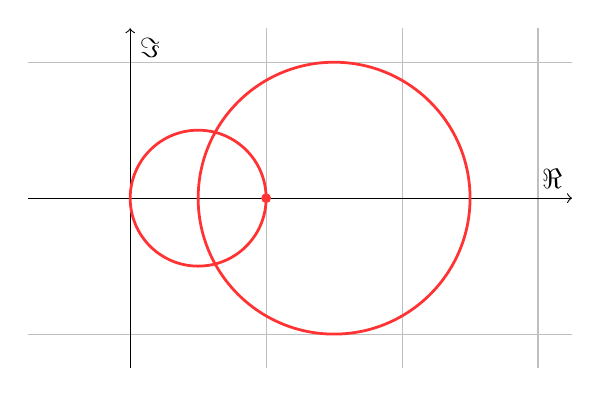
\begin{tikzpicture}
            \begin{axis}[
                    % xtick distance=2,
                    % ytick distance=2,
                    grid=major,
                    % grid style={line width=.1pt, draw=gray!10}%,major grid style={line width=.2pt,draw=gray!50}
                    ticks=none, % ticks aus?
                    axis lines = middle,
                    axis line style={->},
                    ymin=-2.5, ymax=2.5,
                    xmin=-1.5, xmax=6.5,
                    xlabel={$\Re$},
                    ylabel={$\Im$},
                    axis equal image,
                    width=0.7\textwidth
                ]
                \def\circlewidth{1pt}
                % A
                \draw[red!80, line width=\circlewidth] (axis cs:3,0) node[circle=2pt] {} circle (2);
                \draw[red!80, line width=\circlewidth, fill] (axis cs:2,0) circle (0.05);
                \draw[red!80, line width=\circlewidth] (axis cs:1,0) circle (1);

            \end{axis}
        \end{tikzpicture}
    \end{center}

    \[
        A^T =
        \left(
        \begin{array}{ccc}
                \cellcolor{red!20} 3 & \cellcolor{red!10} 0 & \cellcolor{red!10} 1 \\
                \cellcolor{red!10} 1 & \cellcolor{red!20} 2 & \cellcolor{red!10} 0 \\
                \cellcolor{red!10} 1 & \cellcolor{red!10} 0 & \cellcolor{red!20} 1
            \end{array}
        \right)
        \quad \implies \quad
        \begin{matrix}
            \cellcolor{red!20} m_1 = 3 &  & \cellcolor{red!10} r_1 = |0| + |1| = 1 \\
            \cellcolor{red!20} m_2 = 2 &  & \cellcolor{red!10} r_2 = |1| + |0| = 1 \\
            \cellcolor{red!20} m_2 = 1 &  & \cellcolor{red!10} r_3 = |1| + |0| = 1
        \end{matrix}
    \]

    \begin{center}
        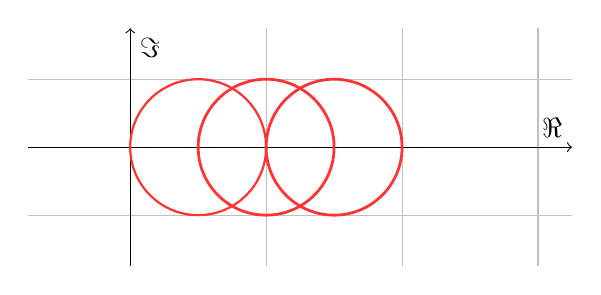
\begin{tikzpicture}
            \begin{axis}[
                    % xtick distance=2,
                    % ytick distance=2,
                    grid=major,
                    % grid style={line width=.1pt, draw=gray!10}%,major grid style={line width=.2pt,draw=gray!50}
                    ticks=none, % ticks aus?
                    axis lines = middle,
                    axis line style={->},
                    ymin=-1.75, ymax=1.75,
                    xmin=-1.5, xmax=6.5,
                    xlabel={$\Re$},
                    ylabel={$\Im$},
                    axis equal image,
                    width=0.7\textwidth
                ]
                \def\circlewidth{1pt}
                % A^T
                \draw[red!80, line width=\circlewidth] (axis cs:3,0) circle (1);
                \draw[red!80, line width=\circlewidth] (axis cs:2,0) circle (1);
                \draw[red!80, thick] (axis cs:1,0) circle (1);

            \end{axis}
        \end{tikzpicture}
    \end{center}
\end{example}

\begin{bonus}{Eigenwertproblem als Nullstellenproblem}
    Ist $A$ symmetrisch, so gelten zusätzlich folgende Aussagen:
    \begin{itemize}
        \item $\lambda_i \in \R, \forall i$
        \item es gibt $n$ Eigenvektoren $v_i$, die linear unabhängig sind, d.h. $A$ ist diagonalisierbar
        \item die $v_i$ können so gewählt werden, dass sie eine Orthonormalbasis bilden:
              \[
                  \langle v_i, v_j \rangle = \delta_{ij}, \quad i, j = 1, \ldots, n
              \]
        \item $Q = \begin{pmatrix}
                      v_1 & \ldots & v_n
                  \end{pmatrix}$ ist eine Orthonormalmatrix und es gilt:
              \[
                  A = Q \Lambda Q^{-1} = Q \Lambda Q^{T}, \quad \Lambda = \begin{pmatrix}
                      \lambda_1 &        &           \\
                                & \ddots &           \\
                                &        & \lambda_n
                  \end{pmatrix}
              \]
              bzw.
              \[
                  \Lambda = Q^T A Q
              \]
        \item da die $v_i$ eine Orthonormalbasis bilden, kann jeder Vektor $x \in \R^n$ geschrieben werden als
              \[
                  x = \sum_{i=1}^{n} x_i v_i, \quad x_i = \langle x, v_i \rangle
              \]
              und
              \[
                  Ax = \sum_{i=1}^{n} x_i A v_i = \sum_{i=1}^{n} \lambda_i x_i v_i
              \]
    \end{itemize}

    Das Eigenwertproblem ist also ein Nullstellenproblem für das Polynom $p_A$.

    Aus der Algebra wissen wir, dass es ab Polynomgrad 5 keinen endlichen Algorithmus zur Lösung dieses Problems gibt.
    Numerische Algorithmen können deswegen nur iterative Verfahren sein.
\end{bonus}

\subsection{Vektoriteration}

\begin{defi}{Vektoriteration}
    Die \emph{Vektoriteration} ist ein numerisches Verfahren zur Berechnung des betragsgrößten Eigenwertes und des dazugehörigen Eigenvektors einer Matrix.

    Wir wissen bereits, dass jedes $x \in \R^n$ als
    \[
        x = \sum_{i=1}^{n} x_i v_i, \quad x_i = \langle x, v_i \rangle
    \]
    geschrieben werden kann.
    Damit gilt:
    \[
        Ax = \sum_i \lambda_i x_i v_i \quad \implies \quad A^kx = \sum_i \lambda_i^k x_i v_i
    \]

    Gilt $|\lambda_1| > \dots > |\lambda_n|$, so dominiert der Anteil $\lambda_1 x_1 v_1$ (falls $x_1 \neq 0$) in $A^k x$.

    Wird $x$ oft genug mit $A$ multipliziert, so bleibt im wesentlichen ein Vielfaches von $v_1$ übrig.

    Ist $|\lambda_1| > 1$, so wird $\|A^kx\|_2$ immer größer.
    Um die damit verbundenen numerischen Probleme zu vermeiden normalisiert man nach jeder Multiplikation mit $A$ den neu berechneten Vektor und erhält somit die \emph{Vektoriteration}:
    \begin{enumerate}
        \item Wähle $x^{(0)}$ mit $\|x^{(0)}\|_2 = 1$ und $x_1^{(0)} = \langle x^{(0)}, v_1 \rangle \neq 0$
        \item Wiederhole:
              \[
                  y^{(k+1)} = A x^{(k)}
              \]
              \[
                  x^{(k+1)} = \frac{y^{(k+1)}}{ \| y^{(k+1)} \|_2 }
              \]
              \[
                  \mu^{(k+1)} = \langle x^{(k)}, y^{(k+1)} \rangle
              \]
    \end{enumerate}

    Ist $A$ symmetrisch mit $\lambda_1 > |\lambda_2| > \dots > |\lambda_n|$.
    Dann ist die Vektoriteration
    \[
        \mu^{(k)} \xrightarrow{k \to \infty} \lambda_1, \quad x^{(k)} \xrightarrow{k \to \infty} \sign(x_1^{(0)}) v_1
    \]
    falls $x_1^{(0)} = \langle x^{(0)}, v_1 \rangle \neq 0$ ist.
\end{defi}

\begin{example}{Vektoriteration}
    Gegeben seien eine Matrix $A$ und ein Startvektor $x^{(0)}$ mit:
    \[
        A =
        \begin{pmatrix}
            2 & 1 & 0 & 0 \\
            1 & 2 & 1 & 0 \\
            0 & 1 & 2 & 1 \\
            0 & 0 & 1 & 2
        \end{pmatrix}
        , \quad
        x^{(0)} =
        \begin{pmatrix}
            1 \\ 0 \\ 0 \\ 0
        \end{pmatrix}
    \]

    Wenden Sie die Vektoriteration an und berechnen Sie den betragsgrößten Eigenwert und den Eigenvektor.

    \exampleseparator

    $k = 1$:
    \[
        y^{(1)} = A x^{(0)} =
        \begin{pmatrix}
            2 & 1 & 0 & 0 \\
            1 & 2 & 1 & 0 \\
            0 & 1 & 2 & 1 \\
            0 & 0 & 1 & 2
        \end{pmatrix}
        \begin{pmatrix}
            1 \\ 0 \\ 0 \\ 0
        \end{pmatrix}
        =
        \begin{pmatrix}
            2 \\ 1 \\ 0 \\ 0
        \end{pmatrix}
    \]
    \[
        x^{(1)} = \frac{y^{(1)}}{ \| y^{(1)} \|_2 } = \frac{1}{\sqrt{5}}
        \begin{pmatrix}
            2 \\ 1 \\ 0 \\ 0
        \end{pmatrix}
        \approx
        \begin{pmatrix}
            0.89 \\ 0.45 \\ 0 \\ 0
        \end{pmatrix}
    \]
    \[
        \mu^{(1)} = \langle x^{(0)}, y^{(1)} \rangle = \langle
        \begin{pmatrix}
            1 \\ 0 \\ 0 \\ 0
        \end{pmatrix},
        \begin{pmatrix}
            2 \\ 1 \\ 0 \\ 0
        \end{pmatrix}
        \rangle
        = 2
    \]

    $k = 2$:
    \[
        y^{(2)} = A x^{(1)} = \frac{1}{\sqrt{5}}
        \begin{pmatrix}
            2 & 1 & 0 & 0 \\
            1 & 2 & 1 & 0 \\
            0 & 1 & 2 & 1 \\
            0 & 0 & 1 & 2
        \end{pmatrix}
        \begin{pmatrix}
            2 \\ 1 \\ 0 \\ 0
        \end{pmatrix}
        = \frac{1}{\sqrt{5}}
        \begin{pmatrix}
            5 \\ 4 \\ 1 \\ 0
        \end{pmatrix}
    \]
    \[
        x^{(2)} = \frac{y^{(2)}}{ \| y^{(2)} \|_2 } = \frac{1}{\sqrt{\frac{42}{5}}} \cdot \frac{1}{\sqrt{5}}
        \begin{pmatrix}
            5 \\ 4 \\ 1 \\ 0
        \end{pmatrix}
        = \frac{1}{\sqrt{42}}
        \begin{pmatrix}
            5 \\ 4 \\ 1 \\ 0
        \end{pmatrix}
        \approx
        \begin{pmatrix}
            0.77 \\ 0.62 \\ 0.15 \\ 0
        \end{pmatrix}
    \]
    \[
        \mu^{(2)} = \langle x^{(1)}, y^{(2)} \rangle = \frac{1}{5} \langle
        \begin{pmatrix}
            2 \\ 1 \\ 0 \\ 0
        \end{pmatrix},
        \begin{pmatrix}
            5 \\ 4 \\ 1 \\ 0
        \end{pmatrix}
        \rangle
        = 2.8
    \]

    $\ldots$

    $k = 15$:
    \[
        x^{(15)} \approx
        \begin{pmatrix}
            0.3793 \\ 0.6061 \\ 0.5968 \\ 0.3641
        \end{pmatrix}
        , \quad
        \mu^{(15)} \approx 3.6177
    \]
\end{example}

\subsection{Jacobi-Verfahren}

\begin{defi}{Jacobi-Verfahren (Eigenwerte)}
    Die Idee des \emph{Jacobi-Verfahrens} besteht darin, das jeweils betragsgrößte Außerdiagonalelement mit Hilfe einer Givens-Rotation auf $0$ zu bringen, und sich auf diese Art mehr und mehr einer Diagonalmatrix anzunähern.

    Es ergibt sich die Iterationsvorschrift:
    \begin{enumerate}
        \item $A^{0} = A$
        \item Wiederhole:
              \[
                  A^{(k+1)} = {Q^{(k)}}^T A^{(k)} Q^{(k)} = \underbrace{Q_k^T \cdot \ldots \cdot Q_1^T}_{{Q^{(k)}}^T} A^{(0)} \underbrace{Q_1 \cdot \ldots \cdot Q_k}_{Q^{(k)}}
              \]
              $Q_k$ wird wie folgt bestimmt:
              \begin{itemize}
                  \item suche das betragsgrößte Nebendiagonalelement $a_{i_0 j_0}^{(k-1)}$ von $A^{k-1}$
                  \item dabei kann $j_0 > i_0$ angenommen werden, da alle Matrizen $A^{k-1}$ symmetrisch sind
                  \item bestimme $Q_k$ so, dass $a_{i_0 j_0}^{(k)} = 0$, also
                        \[
                            Q_k =
                            \begin{pmatrix}
                                1 &        &   &    &   &        &   &   &   &        &   \\
                                  & \ddots &   &    &   &        &   &   &   &        &   \\
                                  &        & 1 &    &   &        &   &   &   &        &   \\
                                  &        &   & c  &   &        &   & s &   &        &   \\
                                  &        &   &    & 1 &        &   &   &   &        &   \\
                                  &        &   &    &   & \ddots &   &   &   &        &   \\
                                  &        &   &    &   &        & 1 &   &   &        &   \\
                                  &        &   & -s &   &        &   & c &   &        &   \\
                                  &        &   &    &   &        &   &   & 1 &        &   \\
                                  &        &   &    &   &        &   &   &   & \ddots &   \\
                                  &        &   &    &   &        &   &   &   &        & 1
                            \end{pmatrix}
                        \]
                        mit
                        \[
                            \alpha = \frac{a_{j_0 j_0} - a_{i_0 i_0}}{2 a_{i_0 j_0}} \quad \implies \quad c = \sqrt{\frac{1}{2} + \frac{1}{2} \sqrt{\frac{\alpha^2}{1 + \alpha^2}}}, \quad s = \frac{\sign(\alpha)}{2c \sqrt{1 + \alpha^2}}
                        \]
              \end{itemize}
    \end{enumerate}

    Dann ist ($\lambda_i$ Eigenwerte, $v_i$ Eigenvektoren)
    \[
        \diagonal(A^{(k)}) =
        \begin{pmatrix}
            a_{11}^{(k)} &        &              \\
                         & \ddots &              \\
                         &        & a_{nn}^{(k)}
        \end{pmatrix}
        \approx
        \begin{pmatrix}
            \lambda_1 &        &           \\
                      & \ddots &           \\
                      &        & \lambda_n
        \end{pmatrix}
        = \Lambda
    \]
    \[
        Q^{(k)} \approx
        \begin{pmatrix}
            v_1 & \ldots & v_n
        \end{pmatrix}
    \]
\end{defi}

\begin{example}{Jacobi-Verfahren}
    Gegeben sei die Matrix $A$ mit:
    \[
        A =
        \begin{pmatrix}
            3 & 4 \\
            4 & 3
        \end{pmatrix}
    \]

    Führen Sie das Jacobi-Verfahren für eine Iteration aus und berechnen Sie die Eigenwerte (näherungsweise).

    \exampleseparator

    \[
        A = A^{(0)} =
        \left(
        \begin{array}{cc}
                3 & \cellcolor{red!20} 4 \\
                4 & 3
            \end{array}
        \right)
        \quad \implies \quad
        i_0 = 1, \quad j_0 = 2
    \]

    Damit gilt:
    \[
        Q_1 =
        \begin{pmatrix}
            c  & s \\
            -s & c
        \end{pmatrix}
    \]
    mit
    \[
        \alpha = \frac{a_{j_0 j_0} - a_{i_0 i_0}}{2 a_{i_0 j_0}} = \frac{a_{22} - a_{11}}{2 a_{1 2}} = \frac{3 - 3}{2 \cdot 4} = 0
    \]
    \[
        \implies \quad c = \sqrt{\frac{1}{2} + \frac{1}{2} \sqrt{\frac{\alpha^2}{1 + \alpha^2}}} = \sqrt{\frac{1}{2}} = \frac{1}{\sqrt{2}}, \quad s = \frac{\sign(\alpha)}{2c \sqrt{1 + \alpha^2}} = \frac{1}{2 \cdot \frac{1}{\sqrt{2}} \cdot \sqrt{1}} = \frac{1}{\sqrt{2}}
    \]
    \[
        \implies \quad Q_1 =
        \left(
        \begin{array}{cc}
                \cellcolor{red!10} \nicefrac{1}{\sqrt{2}}  & \cellcolor{blue!10} \nicefrac{1}{\sqrt{2}} \\
                \cellcolor{red!10} -\nicefrac{1}{\sqrt{2}} & \cellcolor{blue!10} \nicefrac{1}{\sqrt{2}}
            \end{array}
        \right)
    \]
    \[
        \implies \quad A^{(1)} = Q_1^T A^{(0)} Q_1 =
        \begin{pmatrix}
            \nicefrac{1}{\sqrt{2}} & -\nicefrac{1}{\sqrt{2}} \\
            \nicefrac{1}{\sqrt{2}} & \nicefrac{1}{\sqrt{2}}
        \end{pmatrix}
        \begin{pmatrix}
            3 & 4 \\
            4 & 3
        \end{pmatrix}
        \begin{pmatrix}
            \nicefrac{1}{\sqrt{2}}  & \nicefrac{1}{\sqrt{2}} \\
            -\nicefrac{1}{\sqrt{2}} & \nicefrac{1}{\sqrt{2}}
        \end{pmatrix}
        = \ldots =
        \left(
        \begin{array}{cc}
                \cellcolor{red!20} -1 & 0                     \\
                0                     & \cellcolor{blue!20} 7
            \end{array}
        \right)
    \]

    Damit erhalten wir die Eigenwerte und dazugehörigen Eigenvektoren:
    \[
        \lambda_1 = -1, \quad v_1 =
        \begin{pmatrix}
            \nicefrac{1}{\sqrt{2}} \\ -\nicefrac{1}{\sqrt{2}}
        \end{pmatrix}
    \]
    \[
        \lambda_2 = 7, \quad v_2 =
        \begin{pmatrix}
            \nicefrac{1}{\sqrt{2}} \\ \nicefrac{1}{\sqrt{2}}
        \end{pmatrix}
    \]
\end{example}

\subsection{QR-Verfahren, Hessenberg-Transformation, Shift-Technik}

\begin{defi}{QR-Verfahren (singuläre Matrizen)}
    Mit Givens- bzw. Householder-Transformationen können wir eine \emph{reguläre Matrix} $A$ in $A = QR$ zerlegen, wobei $Q$ orthonormal und $R$ eine obere Dreiecksmatrix ist.

    Eine analoge Zerlegung ist auch für \emph{singuläres} $A$ möglich:
    \begin{itemize}
        \item Falls eine Spalte inklusive des Diagonalelements gleich $0$ ist, benutzt man als Dreh- bzw. Spiegelmatrix $Q_k = I$.
        \item Auf der Diagonalen der oberen Dreiecksmatrix $R$ trägt man entsprechend eine $0$ ein.
        \item Wir zerlegen eine beliebige quadratische Matrix $A$ in $A = QR$ und betrachten
              \[
                  RQ = Q^T Q R Q = Q^T A Q
              \]
        \item Da $Q^T = Q^{-1}$ ist, gilt
              \[
                  RQ = Q^{-1} A Q
              \]
              d. h. $RQ$ und $A = QR$ haben die selben Eigenwerte.
        \item Wir bauen daraus wie üblich eine Iteration auf und erhalten das \emph{QR-Verfahren}:
              \begin{enumerate}
                  \item Starte mit $A^{(0)} = A$
                  \item Wiederhole:
                        \begin{enumerate}
                            \item Zerlege
                                  \[
                                      A^{(k)} = Q_k R_k
                                  \]
                            \item Berechne
                                  \[
                                      A^{(k+1)} = R_k Q_k
                                  \]
                        \end{enumerate}
              \end{enumerate}
    \end{itemize}

    Bei symmetrischem $A$ konvergieren die $A^{(k)}$ wie bei Jacobi gegen die Diagonalmatrix $\Lambda$ und die Spalten von $Q^{(k)}$ können wieder als Approximationen der Eigenvektoren benutzt werden.
\end{defi}

\begin{defi}{Hessenberg-Form}
    Eine (obere) \emph{Hessenbergmatrix} ist eine quadratische Matrix $H \in \R^{n \times n}$, deren Einträge unterhalb der ersten Nebendiagonalen gleich Null sind, also $h_{ij} = 0$ für alle $i > j + 1$:
    \[
        H =
        \begin{pmatrix}
            h_{11} & h_{12} & h_{13} & \cdots   & h_{1n} \\
            h_{21} & h_{22} & h_{23} & \cdots   & h_{2n} \\
            0      & h_{32} & h_{33} & \cdots   & h_{3n} \\
            \vdots & \ddots & \ddots & \ddots   & \vdots \\
            0      & \cdots & 0      & h_{nn-1} & h_{nn}
        \end{pmatrix}
    \]

    Analog definiert man die untere Hessenbergmatrix als eine quadratische Matrix, deren Transponierte eine obere Hessenbergmatrix ist.

    Ist nur von einer Hessenbergmatrix die Rede, ist meist eine obere Hessenbergmatrix gemeint.

    Eine Matrix, die sowohl eine untere als auch eine obere Hessenbergmatrix ist, ist eine Tridiagonalmatrix.
\end{defi}

\begin{bonus}{Hessenberg-Form und QR-Verfahren}
    Der Aufwand beim QR-Verfahren entspricht pro Schritt im wesentlichen einer Householder-Zerlegung $(\approx \frac{4}{3} n^3)$ und ist damit extrem hoch.

    Für das QR-Verfahren bringt die Hessenberg-Form folgenden Vorteil:

    Bei der QR-Zerlegung einer Hessenberg-Matrix muss pro Spalte nur das Subdiagonalelement eliminiert werden, was jeweils mit einer einzigen Givens-Rotation erledigt werden kann, so dass der Gesamtaufwand nur noch $\approx n^2$ statt $\approx \frac{4}{3} n^3$ ist.

    Hat $A^{(k)}$ Hessenberg-Form und wurde mit Givens-Matrizen in $A^{(k)} = Q_k R_k$ zerlegt, so hat sowohl $Q_k$ als auch $A^{(k+1)} = R_k Q_k$ wieder Hessenberg-Form.

    Ist $A$ symmetrisch, so vereinfacht sich das ganze nochmals:
    \begin{itemize}
        \item Die Hessenberg-Transformierte $H$ ist wegen $H = QAQ^{-1} = QAQ^T$ ebenfalls symmetrisch und muss deshalb tridiagonal sein.
        \item Wird das QR-Verfahren mit tridiagonalem $A^{(0)}$ gestartet, so sind alle $A^{(k)}$ tridiagonal und der Aufwand für die Zerlegung $A^{(k)} = Q_k R_k$ und die Matrixmultiplikation $Q_k R_k$ ist $\approx n$.
    \end{itemize}
\end{bonus}

\begin{defi}{Hessenberg-Transformation}
    Gegeben sei eine Matrix $A \in \R^{n \times n}$ und $\tilde{A} \in \R^{n-1 \times n}$ eine Untermatrix von $A$, konstruiert durch Entfernen der ersten Zeile von $A$, und $\tilde{a}_1$ die erste Spalte von $\tilde{A}$.

    Wir konstruieren dann die Householder-Matrix $\tilde{Q}_1$, die $\tilde{a}_1$ eliminiert, d.h.
    \[
        \tilde{Q}_1 \tilde{a}_1 = \alpha_1 \begin{pmatrix}
            1 \\ 0 \\ \vdots \\ 0
        \end{pmatrix}
    \]

    Wir erweitern $\tilde{Q}_1$ auf die gesamte orthonormale Matrix $Q_1 \in \R^{n \times b}$, d.h.
    \[
        Q_1 = \begin{bmatrix}
            1 & 0           \\
            0 & \tilde{Q}_1 \\
        \end{bmatrix}
    \]

    Dann gilt
    \[
        Q_1 A = \begin{pmatrix}
            a_{11}   & *      & \cdots & \cdots & *      \\
            \alpha_1 & *      & \cdots & \cdots & *      \\
            0        & \vdots &        &        & \vdots \\
            \vdots   & \vdots &        &        & \vdots \\
            0        & *      & \cdots & \cdots & *
        \end{pmatrix}
        , \quad
        Q_1 A Q_1^T = Q_1 A Q_1^{-1} = \begin{pmatrix}
            a_{11}   & *      & \cdots & \cdots & *      \\
            \alpha_1 & *      & \cdots & \cdots & *      \\
            0        & \vdots &        &        & \vdots \\
            \vdots   & \vdots &        &        & \vdots \\
            0        & *      & \cdots & \cdots & *
        \end{pmatrix}
    \]

    Analoges Vorgehen für Spalte $2$ bis $n-2$ liefert
    \[
        H = \underbrace{Q_{n-2} \cdot \ldots \cdot Q_1}_{Q} A \underbrace{Q_1^T \cdot \ldots \cdot Q_{n-2}^T}_{Q^T = Q^{-1}} = \begin{pmatrix}
            *      & \cdots & \cdots & \cdots & *      \\
            *      & \ddots &        &        & \vdots \\
            0      & \ddots & \ddots &        & \vdots \\
            \vdots & \ddots & \ddots & \ddots & \vdots \\
            0      & \cdots & 0      & *      & *
        \end{pmatrix}
    \]

    $H = Q A Q^{-1}$ hat dieselben Eigenwerte wie $A$ und besitzt Hessenberg-Form, d.h. das um die erste Nebendiagonale reduzierte untere Dreieck ist identisch $0$.
\end{defi}

\begin{example}{Hessenberg-Transformation}
    TODO
\end{example}

\begin{bonus}{QR-Verfahren mit einfachen Shifts}
    Mit der Hessenberg-Transformation haben wir den Aufwand reduziert, aber die Konvergenzgeschwindigkeit kann noch verbessert werden.
    Dazu benutzen wir den folgenden Zusammenhang:

    Zerlege statt $A$ die Matrix
    \[
        A - \mu I = QR
    \]
    Dann hat
    \[
        \tilde{A} = RQ + \mu I
    \]
    wegen $Q^T = Q^{-1}$ dieselben Eigenwerte wie $A$, denn
    % \begin{alignat*}{1}
    %     \tilde{A} & = RQ + \mu I                    \\
    %               & = Q^T Q R Q + \mu I             \\
    %               & = Q^T (A - \mu I) Q + \mu I     \\
    %               & = Q^T A Q - \mu Q^T I Q + \mu I \\
    %               & = Q^T A Q - \mu I + \mu I       \\
    %               & = Q^T A Q
    % \end{alignat*}
    \[
        \tilde{A} = RQ + \mu I = Q^T Q R Q + \mu I = Q^T (A - \mu I) Q + \mu I = Q^T A Q - \mu Q^T I Q + \mu I =  Q^T A Q
    \]

    Damit bauen wir in das QR-Verfahren einen \emph{Shift} ein, d.h. wir ändern die Iteration wie folgt:
    \begin{enumerate}
        \item Starte mit $A^{(0)} = A$ in Hessenberg-Form
        \item Wiederhole:
              \begin{enumerate}
                  \item Zerlege
                        \[
                            A^{(k)} - \mu^{(k)} I = Q_k R_k
                        \]
                  \item Berechne
                        \[
                            A^{(k+1)} = R_k Q_k + \mu^{(k)} I
                        \]
              \end{enumerate}
    \end{enumerate}
    wobei $\mu^{(k)}$ geeignet zu bestimmen ist.

    Üblicherweise wird versucht, mit dem Shift $\mu^{(k)}$ den betragskleinsten Eigenwert $\lambda_n$ zu approximieren.
    Dazu kann das letzte Diagonalelement $\mu^{(k)} = (A^{(k)})_{nn}$ gewählt werden.

    Mit dieser Wahl konvergiert $a^{(k)}_{nn-1}$ schnell gegen $0$ und $a^{(k)}_{nn}$ gegen $\lambda_n$ von $A$, d.h. ist $l > k$ groß genug, dann ist
    \[
        A^{(l)} = \begin{pmatrix}
            *      & \cdots & \cdots & \cdots   & *                 \\
            *      & \ddots &        &          & \vdots            \\
            0      & \ddots & \ddots &          & \vdots            \\
            \vdots & \ddots & *      & *        & *                 \\
            0      & \cdots & 0      & \epsilon & \tilde{\lambda}_n
        \end{pmatrix}
    \]
    wobei $\epsilon \approx 0$ nd $\tilde{\lambda}_n \approx \lambda_n$ ist.

    Damit haben wir einen Eigenwert approximiert und die restlichen Eigenwerte sind ausschließlich durch die ersten $n-1$ Spalten und Zeilen der Matrix bestimmt.
    Deshalb streichen wir die letzte Zeile und Spalte und wiederholen das Verfahren auf der verbliebenen Restmatrix.

    Diese Reduktionstechnik nennt sich \emph{Deflation}.

    Die Implementierung in dieser Form zählt zu den Standardverfahren und findet sich so auch in den einschlägigen Bibliotheken (z.B. \texttt{LAPACK}).

    Die einfache QR-Iteration ergibt sich, indem alle Shifts zu Null gesetzt werden.
\end{bonus}
\section{Nichtlineare Gleichungen}

%\subsection{Einleitung}

\subsection{Einfache Verfahren und ihre geometrische Interpretation}
\subsubsection{Bisektions-Verfahren}

\begin{defi}{Bisektions-Verfahren}
    Wir setzen $f: \R \to \R$ stetig voraus.

    Ist $f(a_0) \cdot f(b_0) < 0$, dann muss in $[a_0, b_0]$ \emph{mindestens} eine Nullstelle von $f$ liegen.

    Betrachte $x_0 = \frac{a_0 + b_0}{2}$, also die Intervallmitte.

    Wiederhole solange, bis die Intervalllänge $|b_i - a_i|$ oder $|f(x_i)|$ hinreichend klein ist:
    \begin{itemize}
        \item Berechne
              \[
                  x_{i} = \frac{a_i + b_i}{2}
              \]
        \item Setze
              \[
                  \begin{cases}
                      a_{i+1} = a_{i}, \quad b_{i+1} = x_{i} & \text{falls } f(x_{i}) \cdot f(a_{i}) < 0 \\
                      a_{i+1} = x_{i}, \quad b_{i+1} = b_{i} & \text{sonst}
                  \end{cases}
              \]
        \item Betrachte nun $[a_{i+1}, b_{i+1}]$
    \end{itemize}

    Das Bisektions-Verfahren ist ein Einschließungsverfahren.
\end{defi}

\begin{example}{Bisektions-Verfahren}
    TODO
\end{example}

\begin{defi}{Einschließungsverfahren}
    Verfahren, die untere und obere Schranken $a_k$ und $b_k$ für eine gesuchte Nullstelle erzeugen, nennt man \emph{Einschließungsverfahren}.
\end{defi}

\subsubsection{Regula-Falsi-Verfahren}

\begin{bonus}{Regula-Falsi-Verfahren (Idee)}
    Wir modifizieren das Bisektions-Verfahren, um die Konvergenzgeschwindigkeit zu erhöhen.

    Benutze für $x_k$ nicht die Intervallmitte, sondern zusätzliche Information:
    \begin{itemize}
        \item verbinde $(a_k, f(a_k))$ und $(b_k, f(b_k))$ durch eine Gerade $s$
        \item $x_k$ sei jetzt die Nullstelle der Geraden $s$ mit
              \[
                  s(x) = f(a_k) + \frac{f(b_k) - f(a_k)}{b_k - a_k} \cdot (x - a_k)
              \]
              \[
                  s(x_k) = 0 \quad \iff \quad x_k = a_k - \frac{b_k - a_k}{f(b_k) - f(a_k)} = \frac{a_k f(b_k) - b_k f(a_k)}{f(b_k) - f(a_k)}
              \]
    \end{itemize}
\end{bonus}

\begin{defi}{Regula-Falsi-Verfahren}
    Das \emph{Regula-Falsi-Verfahren} funktioniert analog zum Bisektions-Verfahren, nur dass $x_k$ wie folgt berechnet wird:
    \[
        x_k = \frac{a_k f(b_k) - b_k f(a_k)}{f(b_k) - f(a_k)}
    \]

    Wiederhole solange, bis die Intervalllänge $|x_{i+1} - x_i|$ oder $|f(x_i)|$ hinreichend klein ist:\footnote{Anderes Abbruchkriterium als beim Bisektions-Verfahren!}
    \begin{itemize}
        \item Berechne
              \[
                  x_{i} = \frac{a_k f(b_k) - b_k f(a_k)}{f(b_k) - f(a_k)}
              \]
        \item Setze
              \[
                  \begin{cases}
                      a_{i+1} = a_{i}, \quad b_{i+1} = x_{i} & \text{falls } f(x_{i}) \cdot f(a_{i}) < 0 \\
                      a_{i+1} = x_{i}, \quad b_{i+1} = b_{i} & \text{sonst}
                  \end{cases}
              \]
        \item Betrachte nun $[a_{i+1}, b_{i+1}]$
    \end{itemize}

    Das Regula-Falsi-Verfahren ist ein Einschließungsverfahren.
\end{defi}

\begin{example}{Regula-Falsi-Verfahren}
    TODO
\end{example}

\subsubsection{Sekanten-Verfahren}

\begin{defi}{Sekanten-Verfahren}
    Wir erhalten das \emph{Sekanten-Verfahren}, indem wir das Regula-Falsi-Verfahren leicht abändern.

    Seien $x_{-2}, x_{-1}$ gegeben.
    Bestimme für $k = 0, 1, \ldots$ die neue Näherung $x_k$ als Nullstelle der Geraden durch die Punkte
    \[
        x_k = x_{k-2} - \frac{x_{k-1} - x_{k-2}}{f(x_{k-1}) - f(x_{k-2}))} \cdot f(x_{k-2}) = x_{k-1} - \frac{x_{k-1} - x_{k-2}}{f(x_{k-1}) - f(x_{k-2}))} \cdot f(x_{k-1})
    \]

    Das Sekanten-Verfahren ist \emph{kein} Einschließungsverfahren.
\end{defi}

\begin{bonus}{Konvergenz des Sekanten-Verfahrens}
    Ist $f$ zweimal stetig differenzierbar in einer hinreichend kleinen Umgebung $X$ der gesuchten Nullstelle $x$.

    Dann konvergiert das Sekanten-Verfahren für alle $x_{-2}, x_{-1} \in X$ und es gibt eine Konstante $c > 0$ so dass
    \[
        |e_k| \leq c |e_{k-1}|^{\frac{1+\sqrt{2}}{2}}, \quad k \to \infty
    \]
\end{bonus}

\subsubsection{Taylor-Reihen-basierte Verfahren, Newton-Verfahren}

\begin{bonus}{Wiederholung Taylor-Entwicklung}
    Ist $f(x) = 0$ und $f$ hinreichend oft differenzierbar, $x_k$ gegeben, so liefert eine Taylor-Entwicklung von $f$ um $x_k$
    \[
        f(y) = f(x_k) + (y - x_k) f'(x_k) + \frac{(y - x_k)^2}{2!} f''(x_k) + \ldots
    \]
    bzw. für $y = x \implies f(y) = 0$
    \[
        0 = f(x) = f(x_k) + (x - x_k) f'(x_k) + \frac{(x - x_k)^2}{2!} f''(x_k) + \ldots
    \]
\end{bonus}

\begin{defi}{Newton-Verfahren}
    Brechen wir die Taylor-Entwicklung nach dem linearen Term ab, dann ist
    \[
        0 = f(x_k) + (\tilde{x} - x_k) f'(x_k) \quad \implies \quad \tilde{x} = x_k - \frac{f(x_k)}{f'(x_k)}
    \]
    und wir erhalten das \emph{Newton-Verfahren} mit
    \[
        x_{k+1} = x_k - \frac{f(x_k)}{f'(x_k)}
    \]

    Geometrisch approximiert das Newton-Verfahren also $f$ durch die Tangente $g$ durch den Punkt $(x_k, f(x_k))$ und benutzt die Nullstelle von $g$ als $x_{k+1}$.

    Brechen wir nach dem quadratischen Term ab so folgt
    \[
        0 = f(x_k) + (\tilde{x} - x_k) f'(x_k) + \frac{(\tilde{x} - x_k)^2}{2} f''(x_k)
    \]
    und damit
    \[
        x_{k+1} = x_k - \frac{f'(x_k) \pm \sqrt{(f'(x_k))^2 - 2 \cdot f(x_k) f''(x_k)}}{f''(x_k)}
    \]

    Hier wird statt einer Tangente eine Parabel $g$ verwendet.
\end{defi}

\begin{example}{Newton-Verfahren}
    TODO
\end{example}

\subsection{Stationäre Iterationen, Banachscher Fixpunktsatz}

\begin{defi}{Picard-Iteration}
    TODO
\end{defi}

\begin{defi}{Kontraktion}
    $\Phi$ heißt \emph{Kontraktion} bezüglich $\| \cdot \|$ auf $X \subset \R^n$ falls
    \begin{enumerate}
        \item $\Phi: X \to X$
        \item $\|\Phi(x) - \Phi(y)\| \leq \alpha \|x-y\|$, $\forall x, y \in X$ und $\alpha , 1$ unabhängig von $x, y$
    \end{enumerate}
\end{defi}

\begin{defi}{Lokale Konvergenz (Iterationen)}
    Die Iteration
    \[
        x_{k+1} = \Phi(x_k)
    \]
    heißt \emph{lokal konvergent} gegen $x \in X \subset \R^n$ falls
    \[
        \lim_{k \to \infty} x_k = x \quad \forall x_0 \in X
    \]
\end{defi}

\begin{defi}{Banachscher Fixpunktsatz}
    Sei $X \subset \R^n$ abgeschlossen und $\Phi: X \to X$ eine Kontraktion auf $X$ mit
    \[
        \|\Phi(x) - \Phi(y)\| \leq \alpha \|x-y\| \quad x, y \in X, \alpha < 1
    \]

    Dann hat $\Phi$ genau einen Fixpunkt mit $x = \Phi(x)$ in $X$.

    Die Picard-Iteration
    \[
        x_{k+1} = \Phi(x_k)
    \]
    konvergiert $\forall x_0 \in X$ gegen $x$.
    Es gelten die Abschätzungen
    \[
        \|x - x_k\| \leq \frac{\alpha^k}{1-\alpha} \|x_1 - x_0\| \qquad \text{\emph{a-priori Abschätzung}}
    \]
    \begin{itemize}
        \item $\|e_k\|$ kann allein mit $\alpha, x_0, x_1$ abgeschätzt werden, ohne ausrechnen von $x_k$
        \item wird benutzt um maximale Zahl der Iterationen für gegebene Genauigkeit zu bestimmen
        \item oft sehr grob
    \end{itemize}

    \[
        \|x - x_k\| \leq \frac{\alpha}{1-\alpha} \|x_k - x_{k-1}\| \qquad \text{\emph{a-posteriori Abschätzung}}
    \]
    \begin{itemize}
        \item $\|e_k\|$ kann mit $\alpha, x_k, x_{k-1}$ erst abgeschätzt werden, wenn $x_k$ berechnet wurde
        \item in der Regel genauer als a-priori Abschätzung
        \item oft als Abbruchkriterium genutzt
    \end{itemize}

    Es gilt:
    \begin{itemize}
        \item ist $\Phi$ eine Kontraktion, so existiert genau ein Fixpunkt
        \item $x_k$ konvergiert gegen $x$
        \item Kontraktion $\implies$ Konvergenz
        \item in der Regel erhält man nur lokale Konvergenz ($X \neq \R^n$)
    \end{itemize}
\end{defi}


\begin{example}{Banachscher Fixpunktsatz}
    TODD
\end{example}

\begin{defi}{Konvergenzgeschwindigkeit}
    \index{Lineare Konvergenz}
    \index{Konvergenzordnung}
    %
    Die Iteration $x_{k+1} = \Phi(x_k)$ heißt
    \begin{itemize}
        \item \emph{linear konvergent}, falls es eine Konstante $0 \leq c < 1$ unabhängig von $k$ gibt mit
              \[
                  \|e_{k+1}\| \leq c \|e_k\| \quad \forall k
              \]
        \item \emph{konvergent mit Ordnung} $m$, falls es eine Konstante $0 \leq c$ unabhängig von $k$ gibt mit
              \[
                  \lim_{k \to \infty} \|e_k\| = 0 \quad \land \quad \|e_{k+1}\| \leq c \|e_k\|^m \quad \forall k
              \]
              \begin{itemize}
                  \item Ist $m > 1$, so nennt man $\Phi$ \emph{superlinear konvergent}.
                  \item Für $m = 2$ erhalten wir \emph{quadratische Konvergenz}.
              \end{itemize}
    \end{itemize}
\end{defi}

\begin{bonus}{Konvergenzgeschwindigkeit stetig differenzierbarer Funktionen}
    Ist $m \geq 2$, $x$ ein Fixpunkt von $\Phi: \R \to \R$ und $\Phi$ $m$-mal stetig differenzierbar in $x$ mit
    \[
        \Phi'(x) = \Phi''(x) = \cdots = \Phi^{(m-1)}(x) = 0
    \]
    dann gibt es ein abgeschlossenes Intervall $X = [ x - \delta, x + \delta ]$, $\delta > 0$, so dass die Iteration
    \[
        x_{k+1} = \Phi(x_k)
    \]
    für alle $x_0 \in X$ \text{mindestens mit Ordnung $m$ konvergiert}.


    Ist $m \geq 2$, $x$ ein Fixpunkt von $\Phi: \R \to \R$ und $\Phi$ $(m-1)$-mal stetig differenzierbar in $x$ mit
    \[
        \Phi'(x) = \Phi''(x) = \cdots = \Phi^{(m-1)}(x) = 0, \quad \Phi^{(m)} \neq 0
    \]
    dann gibt es ein abgeschlossenes Intervall $X = [ x - \delta, x + \delta ]$, $\delta > 0$, so dass die Iteration
    \[
        x_{k+1} = \Phi(x_k)
    \]
    für alle $x_0 \in X$ \text{genau mit Ordnung $m$ konvergiert}.
\end{bonus}

\subsection{Newton-Verfahren}
\section{Interpolation}

\subsection{Einleitung}

\begin{defi}{Interpolation}
    Der Begriff \emph{Interpolation} bescheibt eine Klasse von Problemen und Verfahren. 
    
    Zu gegebenen diskreten Daten (z. B. Messwerten) soll eine stetige Funktion (die sogenannte \emph{Interpolante} oder \emph{Interpolierende}) gefunden werden, die diese Daten abbildet. 
    
    Man sagt dann, die Funktion \emph{interpoliert} die Daten. 
\end{defi}

\subsection{Polynominterpolation}

\begin{defi}{Vandermonde-Matrix}
    Die \emph{Vandermonde-Matrix} spielt bei der Interpolation von Funktionen eine wichtige Rolle: 
    
    Wenn an den Stützstellen $(x_0, x_1, \ldots, x_n)$ die Funktionswerte $(y_0, y_1, \ldots, y_n)$ durch ein Polynom $p$ vom Grad $n$ (oder kleiner) interpoliert werden sollen, dann führt der Ansatz 
    \[
        p_n(x) = a_0 + a_1 x^1 + a_2 x^2 + \ldots + a_{n} x^{n}
    \]
    auf das lineare Gleichungssystem 
    \[
        \underbrace{\begin{pmatrix}
                1      & x_0    & \cdots & x_0^n  \\ 
                \vdots & \vdots &        & \vdots \\ 
                1      & x_n    & \cdots & x_n^n 
            \end{pmatrix}}_{V(x_0, \ldots, x_n)}
        \underbrace{\begin{pmatrix}
                a_0 \\ \vdots \\ a_n
            \end{pmatrix}}_{\alpha}
        =
        \underbrace{\begin{pmatrix}
                y_0 \\ \vdots \\ y_n     
            \end{pmatrix}}_{y}
    \]
    mit einer Vandermonde-Matrix $Vx_0, \ldots, x_n)$ als Koeffizientenmatrix.\footnote{Beachte: Für ein Polynom vom Grad $n$ haben wir $n+1$ Koeffizienten!}
    
    Ist $x_i \neq x_j$ ($\forall i \neq j$) so gibt es genau ein Polynom $p_n(x)$ mit Grad $\leq n$, das $(x_0, y_0), \ldots, (x_n, y_n)$ interpoliert. 
\end{defi}

\begin{defi}{Vandermonde-Determinante}
    Die Determinante der Vandermonde-Matrix wird auch \emph{Vandermonde-Determinante} genannt.
    Sie hat den Wert 
    \[
        \det V(x_0, \ldots, x_n) = \prod_{1 \leq i < j \leq n} (x_j - x_i)
    \]
    
    Insbesondere ist die Vandermonde-Matrix genau dann regulär, wenn die $x_i$ paarweise verschieden sind. 
\end{defi}

\begin{defi}{Horner-Schema}
    Um Zwischenstellen eines Polynoms $p_n(x)$ auszuwerten, nutzt man in der Regel nicht direkt die Form 
    \[
        p_n(x) = a_0 + a_1 x + \ldots + a_n x^n    
    \]
    Diese Auswertung ist teuer und durch die vielen Summationen sehr anfällig für Rundungsfehler.
    
    Besser ist hier das \emph{Horner-Schema}: 
    \begin{itemize}
        \item $p_n(x)$ wird wie folgt umgeformt:
              \begin{alignat*}{1}
                  p_n (x) & = a_0 + a_1 x + a_2 x^2 + \ldots + a_n x^n                                                                                                                                                      \\ 
                          & = a_0 + x \left( a_1 + a_2 x + \ldots + a_n x^{n-1} \right)                                                                                                                                     \\ 
                          & = a_0 + x \left( a_1 + x \left( a_2 + \ldots + a_n x^{n-2} \right) \right)                                                                                                                      \\ 
                          & = \ \ldots                                                                                                                                                                                      \\ 
                          & = \underbrace{a_0 + x \underbrace{( a_1 + x \underbrace{( a_2 + x \underbrace{( \ldots + x \underbrace{( a_{n-1} + x \underbrace{a_n}_{q_0} )}_{q_1} )}_{\ldots} )}_{q_{n-2}} )}_{q_n-1}}_{q_n}
              \end{alignat*}
        \item Berechne schrittweise von innen nach außen:
              \begin{alignat*}{1}
                  q_0 & = a_n                   \\ 
                  q_1 & = a_{n-1} + x \cdot q_0 \\
                  q_2 & = a_{n-2} + x \cdot q_1 \\
                      & \ldots
              \end{alignat*}
              also
              \[ 
                  q_0 = a_n, \quad q_k = a_{n-k} + x \cdot q_{k-1}, \quad k = 1, \ldots, n
              \]
              und damit 
              \[ 
                  p_n(x) = q_n
              \]
    \end{itemize}
\end{defi}

\begin{defi}{Lagrange-Polynom}
    Wir betrachten $x_0, \ldots, x_n$ und definieren das $j$-te \emph{Lagrange-Polynom} als 
    \[ 
        L_j(x) = \frac{x - x_0}{x_j - x_0} \cdot \frac{x - x_{j-1}}{x_j - x_{j-1}} \cdot \frac{x - x_{j+1}}{x_j - x_{j+1}} \cdot \ldots \cdot \frac{x - x_n}{x_j - x_n}
    \]
    
    $L_j$ ist wohldefiniert, wenn die $x_i$ paarweise verschieden sind und hat Grad $n$.
    
    Außerdem gilt 
    \[
        L_j(x_i) = 
        \begin{cases}
            1 & \text{für} \ i = j \\ 
            0 & \text{sonst}
        \end{cases}
    \]
    
    Mit den Lagrange-Polynomen $L_j$ können wir das Interpolationspolynom einfach ermitteln mit 
    \[
        p_n(x) = \sum_{j = 0}^{n} y_j \cdot L_j(x)    
    \]
    
    Bei der Benutzung der Lagrange-Polynome muss kein Gleichungssystem gelöst werden, allerdings müssen sämtliche $L_j$ verändert werden, wenn ein weiterer Datenpunkt hinzukommt.
\end{defi}

\begin{example}{Lagrange-Polynom}
    Gegeben seien die folgenden Datenpunkte: 
    
    \begin{center}
        \begin{tabular}{|c||c|c|c|c|}
            \hline
            $x_i$ & -1 & 0 & 1 & 2 \\ 
            \hline
            $y_i$ & 2  & 2 & 2 & 8 \\
            \hline
        \end{tabular}
    \end{center}
    
    Berechnen Sie das zugehörige Lagrange-Interpolationspolynom.
    
    \exampleseparator
    
    Die Lagrange-Polynome sind wie folgt: 
    \[ 
        L_0(x) = \frac{x - x_1}{x_0 - x_1} \cdot \frac{x - x_2}{x_0 - x_2} \cdot \frac{x - x_3}{x_0 - x_3} = \frac{x - 0}{-1 - 0} \cdot \frac{x - 1}{-1 - 1} \cdot \frac{x - 2}{-1 - 2} = -\frac{x(x-1)(x-2)}{6}
    \]
    \[ 
        L_1(x) = \frac{x - x_0}{x_1 - x_0} \cdot \frac{x - x_2}{x_1 - x_2} \cdot \frac{x - x_3}{x_1 - x_3} = \frac{x - (-1)}{0 - (-1)} \cdot \frac{x - 1}{0 - 1} \cdot \frac{x - 2}{0 - 2} = \frac{(x+1)(x-1)(x-2)}{2}
    \]
    \[ 
        L_2(x) = \frac{x - x_0}{x_2 - x_0} \cdot \frac{x - x_1}{x_2 - x_1} \cdot \frac{x - x_3}{x_2 - x_3} = \frac{x - (-1)}{1 - (-1)} \cdot \frac{x - 0}{1 - 0} \cdot \frac{x - 2}{1 - 2} = -\frac{(x+1)x(x-2)}{2}
    \]
    \[ 
        L_3(x) = \frac{x - x_0}{x_3 - x_0} \cdot \frac{x - x_1}{x_3 - x_1} \cdot \frac{x - x_2}{x_3 - x_2} = \frac{x - (-1)}{2 - (-1)} \cdot \frac{x - 0}{2 - 0} \cdot \frac{x - 1}{2 - 1} = \frac{(x+1)x(x-2)}{6}
    \]
    
    Damit ist das Lagrange-Interpolationspolynom $p(x)$: 
    \begin{alignat*}{1}
        p(x) = \quad & y_0 L_0 + y_1 L_1 + y_2 L_2 + y_3 L_3                                                                  \\
        =      \quad & -\frac{2x(x-1)(x-2)}{6} + \frac{2(x+1)(x-1)(x-2)}{2} - \frac{2(x+1)x(x-2)}{2} + \frac{8(x+1)x(x-2)}{6} \\ 
        =      \quad & \ldots                                                                                                 \\ 
        =      \quad & x^3 - x + 2
    \end{alignat*}
\end{example}

\begin{defi}{Newton-Interpolationspolynom}
    \index{Methode der dividierten Differenzen}
    %
    Ein \emph{Newton-Interpolationspolynom} ist ein Interpolationspolynom für eine bestimmte Menge von Datenpunkten.
    
    Gegeben seien $n+1$ paarweise verschiedene Datenpunkte $(x_0, y_0), \ldots, (x_n, y_n)$.
    
    Das \emph{Newton-Interpolationspolynom} ist dann eine Linearkombination der Newton-Basispolynome $N_j(x)$ mit 
    \[ 
        p_n(x) = \sum_{j=0}^{n} a_j N_j(x)  
    \]
    \[  
        = a_0 + a_1 (x - x_0) + a_2 (x - x_0) (x - x_1) + \ldots + a_n (x - x_0) \cdot \ldots \cdot (x - x_{n-1})
    \]
    wobei 
    \[
        N_j (x) = \prod_{i=0}^{j-1} \left( x - x_i \right)
    \]
    
    Die $a_j$ lassen sich wie folgt mithilfe der \emph{Methode der dividierten Differenzen} berechnen.
    
    Es gilt 
    \[ 
        a_j = d_{n, 0}, \quad j = 0, \ldots, n
    \]
    
    Dabei ist 
    \[ 
        d_{n, m} = \frac{d_{n, m+1} - d_{n-1, m}}{x_n - x_m}, \quad n > m
    \]
    mit 
    \[
        d_{i,i} = y_i, \quad i = 0, 1, \ldots    
    \]
    
    Bei gegebenen Punkten $(x_i, y_i)$ kann damit punktweise (Zeile für Zeile) folgendes Schema aufgebaut werden:
    \[
        \begin{array}{cccccccccccccc}
            y_0     & = & d_{0,0}      & =           & a_0                                                                                                              \\
                    &   &              & \searrow                                                                                                                       \\
            y_1     & = & d_{1,1}      & \rightarrow & d_{1,0}      & =           & a_1                                                                                 \\
                    &   &              & \searrow    &              & \searrow                                                                                          \\
            y_2     & = & d_{2,2}      & \rightarrow & d_{2,1}      & \rightarrow & d_{2,0}      & =      & a_2                                                         \\
            \vdots  &   &              & \vdots      & \vdots       & \vdots      & \vdots       & \ddots                                                               \\
            y_{n-1} & = & d_{n-1, n-1} & \rightarrow & d_{n-1, n-2} & \rightarrow & d_{n-1, n-3} & \cdots & \rightarrow & d_{n-1, 0} & =           & a_{n-1}            \\
                    &   &              & \searrow    &              & \searrow    &              &        & \searrow    &            & \searrow                         \\
            y_n     & = & d_{n,n}      & \rightarrow & d_{n, n-1}   & \rightarrow & d_{n, n-2}   & \cdots & \rightarrow & d_{n, 1}   & \rightarrow & d_{n, 0} & = & a_n
        \end{array}
    \]
    
    Wird ein Punkt hinzugefügt, wird das Schema lediglich um eine Zeile erweitert.
    
    Insgesamt ist das Newton-Interpolationspolynom also gegeben mit 
    \[ 
        p_n(x) = \sum_{j=0}^{n} d_{j,0} N_j(x)  
    \]
    \[  
        = d_{0, 0} + d_{1, 0} (x - x_0) + d_{2, 0} (x - x_0) (x - x_1) + \ldots + d_{n, 0} (x - x_0) \cdot \ldots \cdot (x - x_{n-1})
    \]
\end{defi}

\begin{example}{Newton-Interpolationspolynom}
    Gegeben seien die folgenden Datenpunkte: 
    
    \begin{center}
        \begin{tabular}{|c||c|c|c|c|}
            \hline
            $x_i$ & -1 & 0 & 1 & 2 \\ 
            \hline
            $y_i$ & 2  & 2 & 2 & 8 \\
            \hline
        \end{tabular}
    \end{center}
    
    Berechnen Sie das zugehörige Newton-Interpolationspolynom.
    
    \exampleseparator
    
    Das Newton-Interpolationspolynom ist:
    \[ 
        p_3(x) = \sum_{j=0}^{3} d_{j,0} N_j(x) 
    \]
    \[ 
        = a_0 + a_1 (x - x_0) + a_2 (x - x_0) (x - x_1) + a_3 (x - x_0) (x - x_1) (x - x_2) 
    \]
    
    Es gilt:
    
    {
    \footnotesize
    \[
        \begin{array}{llllllllllll}
            y_0 & = & d_{0,0} = 2 & =           & a_0                                                                                                                                                                                                              \\
                &   &             & \searrow                                                                                                                                                                                                                       \\
            y_1 & = & d_{1,1} = 2 & \rightarrow & d_{1,0} = \frac{d_{1,1} - d_{0,0}}{x_1 - x_0} = \frac{2 - 2}{0 + 1} = 0 & =           & a_1                                                                                                                      \\
                &   &             & \searrow    &                                                                         & \searrow                                                                                                                               \\
            y_2 & = & d_{2,2} = 2 & \rightarrow & d_{2,1} = \frac{d_{2,2} - d_{1,1}}{x_2 - x_1} = \frac{2 - 2}{1 - 0} = 0 & \rightarrow & d_{2,0} = \frac{d_{2,1} - d_{1,0}}{x_2 - x_0} = \frac{0 - 0}{1 + 1} = 0  & =           & a_2                             \\
                &   &             & \searrow    &                                                                         & \searrow    &                                                                          & \searrow                                      \\
            y_3 & = & d_{3,3} = 8 & \rightarrow & d_{3,2} = \frac{d_{3,3} - d_{2,2}}{x_3 - x_2} = \frac{8 - 2}{2 - 1} = 6 & \rightarrow & d_{3, 1} = \frac{d_{3,2} - d_{2,1}}{x_3 - x_1} = \frac{6 - 0}{2 - 0} = 3 & \rightarrow & d_{3, 0} = \ldots = 1 & = & a_3 \\
        \end{array}
    \]
    }
    
    Damit ist: 
    \[ 
        p_3(x) = 2 + 1 (x - x_0) (x - x_1) (x - x_2) = 2 + (x+1) x (x-1) = 2 + x(x^2 - 1) = 2 - x + x^3
    \]
    \qed
\end{example}

\subsection{Splines}

\begin{defi}{Polynom-Spline}
    Gegeben seien eine natürliche Zahl $n \in \N$ und $n+1$ Stützstellen $x_0 < x_1 < \ldots < x_{n} \in \R$ sowie $n+1$ Funktionswerte $y_0, y_1, \ldots, y_n \in \R$. 
    
    Gesucht ist eine stückweise polynomiale Funktion, ein \emph{Polynom-Spline}
    \[ 
        S: [x_0, x_n] \to \R
    \]
    mit $S(x_i) = y_i$ für $i = 0, 1, \ldots, n-1$, bei der für $i = 0, \ldots, n-1$ die Teilfunktionen 
    \[
        s_i := S|_{[x_{i},x_{i+1}]} : [x_i, x_{i+1}] \to \R
    \]
    auf die Teilintervalle $[x_{i}, x_{i+1}]$ Polynome sind.
\end{defi}

\begin{bonus}{Polygonzug}
    Bei Polynomgrad $\leq 1$ auf $[x_i, x_{i+1}]$ und stetigen Übergängen erhalten wir einen interpolierenden \emph{Polygonzug}.
    
    TODO Grafik von Folie 495
    
    Es gilt: 
    \[ 
        s_i(x) = mx + b = \underbrace{\frac{y_{i+1} - y_i}{x_{i+1} - x_i}}_{= m} \cdot x + \underbrace{y_i - \frac{y_{i+1} - y_i}{x_{i+1} - x_i} \cdot x_i}_{= b = y_i - m \cdot x_i}
    \]
\end{bonus}

\begin{defi}{Kubischer Polynom-Spline}
    In der Praxis werden \emph{kubische Polynom-Splines} ($k = 3$) am häufigsten benutzt:
    \[ 
        s_i := S_3|_{[x_i, x_{i+1}]} = a_i + b_i x + c_i x^2 + d_i x^3
    \]
    
    $S_3$ ist zweimal stetig differenzierbar auf $[x_0, x_n]$, also insbesondere an den Nahtstellen $x_i$, $i = 1, \ldots, n-1$.
    
    Wir haben $n$ Intervalle $[x_i, x_{i+1}]$, $i = 0, \ldots, n-1$, so dass $4n$ Koeffizienten $a_i, b_i, c_i, d_i$ zu bestimmen sind für die $n$ Polynome $s_i$. 
    
    Für alle kubischen Polynom-Splines gelten folgende Bedingungsgleichungen: 
    \begin{itemize}
        \item $2n$ Bedingungen für die Interpolation:
              \begin{alignat*}{1}
                  s_0(x_0)         & = y_0     \\
                  s_0(x_1)         & = y_1     \\
                  s_1(x_1)         & = y_1     \\
                  s_1(x_2)         & = y_2     \\
                  s_2(x_2)         & = y_2     \\
                  \vdots           &           \\
                  s_{n-1}(x_{n-1}) & = y_{n-1} \\
                  s_{n-1}(x_n)     & = y_n     \\
              \end{alignat*}
        \item $n-1$ Glattheitsbedingungen für die erste Ableitung:
              \begin{alignat*}{1}
                  s'_0(x_1)         & = s'_1(x_1)         \\
                  s'_1(x_2)         & = s'_2(x_2)         \\
                  \vdots            &                     \\
                  s'_{n-2}(x_{n-1}) & = s'_{n-1}(x_{n-1}) \\
              \end{alignat*}
        \item $n-1$ Glattheitsbedingungen für die zweite Ableitung:
              \begin{alignat*}{1}
                  s''_0(x_1)         & = s''_1(x_1)         \\
                  s''_1(x_2)         & = s''_2(x_2)         \\
                  \vdots             &                      \\
                  s''_{n-2}(x_{n-1}) & = s''_{n-1}(x_{n-1}) \\
              \end{alignat*}
    \end{itemize}
    
    Damit haben wir $4n-2$ Gleichungen für $4n$ Unbekannte und brauchen zwei zusätzliche \emph{Abschlussbedingungen}.
\end{defi}

\begin{bonus}{Moment (Idee)}
    Die zweite Ableitung eines kubischen Splines $S_3$ ist ein linearer Spline (Polygonzug). 
    
    Dieser kann wie folgt berechnet werden: 
    \[ 
        s''_i = \frac{x_{i+1} - x}{h_i} \cdot \beta_i + \frac{x - x_i}{h_i} \cdot \beta_{i-1}, \quad h_i = x_{i+1} - x_i, \quad i = 1, \ldots, n-1
    \]
    
    $\beta_i$ sind die sogenannten \emph{Momente}, welche den Werten von $S''(x_i)$ an den Stützstellen entsprechen und noch zu berechnen sind. 
    
    Durch zweifache Integration entstehen aus diesen Gleichungen Polynome dritten Grades mit zwei Parametern $c_i$ und $d_i$ der Form: 
    \[ 
        \frac{1}{6} \left( \frac{(x_{i+1} - x)^3}{h_i} \cdot \beta_i + \frac{(x - x_i)^3}{h_i} \cdot \beta_{i+1} \right) + c_i \cdot (x - x_i) + d_i
    \]
    
    Um die Stetigkeitsbedingungen $s_i(x_i) = y_i$ und $s_i(x_{i+1}) = y_{i+1}$ zu erfüllen, wählen wir
    \[
        d_i = y_i - \frac{h_i^2}{6}, \quad c = \frac{y_{i+1} - y_i}{h_i} - \frac{h_i}{6} \cdot (\beta_{i+1} - \beta_i)
    \]
    
    So sind bereits die nullten und die zweiten Ableitungen der Einschränkungen $s_i$ an den Stützstellen korrekt.
    Die Momente sind so zu wählen, dass auch die ersten Ableitungen an den Stützstellen gleich sind. 
    
    Mit
    \[ 
        s'_i(x) = \frac{1}{2} \left( - \frac{(x_{i+1} - x)^2}{h_i} \cdot \beta_i + \frac{(x - x_i)^2}{h_i} \cdot \beta_{i+1} \right) + c_i 
    \]
    und 
    \[ 
        s'_i(x_i) = s'_{i-1}(x_i)    
    \]
    lassen sich folgende Gleichungen aufstellen: 
    \[
        \frac{h_{i-1}}{6} \cdot M_{i-1} + \frac{h_{i-1}+h_{i}}{3} \cdot \beta_{i} + \frac{h_{i}}{6} \cdot \beta_{i+1} = \frac{y_{i+1}-y_{i}}{h_{i}} - \frac{y_{i}-y_{i-1}}{h_{i-1}}
    \]
    
    Für $i = 0$ und $i = n$ fehlen zwei Gleichungen, die sich aus den \emph{Abschlussbedingungen} ergeben.
    
    Dieses lineare Gleichungssystem kann auch durch folgende, tridiagonale, streng diagonaldominante Matrix ausgedrückt werden: 
    \[
        \begin{pmatrix}
            \mu_{0}         & \lambda_{0}           &                   &                         &                  &          \\
            \frac{h_{0}}{6} & \frac{h_{0}+h_{1}}{3} & \frac {h_{1}}{6}  &                         &                  &          \\
                            & \ddots                & \ddots            & \ddots                  &                  &          \\
                            &                       & \frac{h_{i-1}}{6} & \frac{h_{i-1}+h_{i}}{3} & \frac {h_{i}}{6} &          \\
                            &                       &                   & \ddots                  & \ddots           & \ddots   \\
                            &                       &                   &                         & \lambda _{n}     & \mu _{n}
        \end{pmatrix}
        \cdot 
        \begin{pmatrix}
            M_{0} \\ M_{1} \\ \vdots \\ M_{i} \\ \vdots \\ M_{n}
        \end{pmatrix}
        =
        \begin{pmatrix}
            b_{0}                                                       \\
            \frac{y_{2}-y_{1}}{h_{1}} - \frac{y_{1}-y_{0}}{h_{0}}       \\
            \vdots                                                      \\
            \frac{y_{i+1}-y_{i}}{h_{i}} - \frac{y_{i}-y_{i-1}}{h_{i-1}} \\
            \vdots                                                      \\
            b_{n}
        \end{pmatrix}
    \]
    Die Werte für die $\lambda_i$, $\mu_i$ und $b_i$ hängen von den Abschlussbedingungen ab.
\end{bonus}

\begin{defi}{Berechnung eines kubischen Polynom-Splines}
    Berechne aus $x_i$ die $h_i = x_{i+1} - x_i$ und stelle das lineare Gleichungssystem 
    \[
        \underbrace{
            \begin{pmatrix}
                \mu_{0}         & \lambda_{0}           &                   &                         &                  &          \\
                \frac{h_{0}}{6} & \frac{h_{0}+h_{1}}{3} & \frac {h_{1}}{6}  &                         &                  &          \\
                                & \ddots                & \ddots            & \ddots                  &                  &          \\
                                &                       & \frac{h_{i-1}}{6} & \frac{h_{i-1}+h_{i}}{3} & \frac {h_{i}}{6} &          \\
                                &                       &                   & \ddots                  & \ddots           & \ddots   \\
                                &                       &                   &                         & \lambda _{n}     & \mu _{n}
            \end{pmatrix}
        }_{A}
        \cdot 
        \underbrace{
            \begin{pmatrix}
                M_{0} \\ M_{1} \\ \vdots \\ M_{i} \\ \vdots \\ M_{n}
            \end{pmatrix}
        }_{x}
        =
        \underbrace{
            \begin{pmatrix}
                b_{0}                                                       \\
                \frac{y_{2}-y_{1}}{h_{1}} - \frac{y_{1}-y_{0}}{h_{0}}       \\
                \vdots                                                      \\
                \frac{y_{i+1}-y_{i}}{h_{i}} - \frac{y_{i}-y_{i-1}}{h_{i-1}} \\
                \vdots                                                      \\
                b_{n}
            \end{pmatrix}
        }_{b}
    \]
    auf. 
    Die Werte für die $\lambda_i$, $\mu_i$ und $b_i$ hängen von den Abschlussbedingungen ab.\footnote{Wir betrachten meist \emph{natürliche Splines}, also $\lambda_0 = \lambda_n = b_0 = b_n = 0, \quad \mu_0 = \mu_n = 1$.}
    
    $A$ ist symmetrisch, tridiagonale und streng diagonaldominant, also sehr einfach mit direkten oder iterativen Lösern zu bearbeiten. 
    
    Löse das lineare Gleichungssystem.
    
    Dann ist $s_i(x)$ auf dem Teilintervall $[x_i, x_{i+1}]$ gegeben mit
    \[ 
        s_i(x) = \alpha_i + \beta_i (x - x_{i}) + \gamma_i (x - x_{i})^2 + \delta_i (x - x_{i})^3
    \]
    wobei
    \begin{alignat*}{1}
        \alpha_i & = y_i                                                        \\ 
        \beta_i  & = \frac{y_{i+1} - y_i}{h_i} - \frac{h_i}{6} (2M_i + M_{i+1}) \\
        \gamma_i & = \frac{M_{i}}{2}                                            \\ 
        \delta_i & = \frac{M_{i+1} - M_{i}}{6 h_i}
    \end{alignat*}
\end{defi}

\begin{defi}{Abschlussbedingungen für kubische Polynom-Splines}
    Prinzipiell gibt es ein Interpolationsintervall weniger als Stützstellen. 
    Das heißt, dass zwei Gleichungen zur Bestimmung aller Koeffizienten fehlen. 
    
    Typische \emph{Abschlussbedingungen} sind: 
    \begin{itemize}
        \item \emph{Natürlicher Spline} (freier Rand):
              \begin{itemize}
                  \item Bedingung:
                        \begin{alignat*}{1}
                            s''_0(x_0)     & = 0 \\
                            s''_{n-1}(x_n) & = 0
                        \end{alignat*}
                  \item Der Spline schließt mit Wendepunkten ab.
                  \item Berechnung mit Momenten:
                        \[
                            \lambda_0 = \lambda_n = b_0 = b_n = 0, \quad \mu_0 = \mu_n = 1
                        \]
              \end{itemize}
        \item \emph{Hermiter Spline} (eingespannter Rand):
              \begin{itemize}
                  \item Bedingung:
                        \begin{alignat*}{1}
                            s'_0(x_0)     & = f'(a) \\
                            s'_{n-1}(x_n) & = f'(b)
                        \end{alignat*}
                  \item $f'(a)$ und $f'(b)$ sind vorgegeben, normalerweise entweder durch die Ableitung einer zu interpolierenden Funktion $f$ oder durch eine Approximation derselben.
                  \item Berechnung mit Momenten:
                        \[
                            \lambda_0 = \frac{h_0}{6}, \quad \mu_0 = \frac{h_0}{3}, \quad b_0 = \frac{y_1 - y_0}{h_0} - f'(a)
                        \]
                        \[
                            \lambda_n = \frac{h_{n-1}}{6}, \quad \mu_n = \frac{h_{n-1}}{3}, \quad b_n = - \frac{y_n - y_{n-1}}{h_{n-1}} + f'(b)
                        \]
              \end{itemize}
        \item \emph{Periodischer Spline}:
              \begin{itemize}
                  \item Bedingung:
                        \begin{alignat*}{1}
                            s'_0(x_0)  & = s'_{n-1}(x_n)  \\
                            s''_0(x_0) & = s''_{n-1}(x_n) \\
                        \end{alignat*}
                  \item Nullte, erste und zweite Ableitung von $S_3$ am Anfang und Ende des Intervalls gleich.
                  \item Berechnung mit Momenten:
                        \[
                            \lambda_0 = \frac{h_0}{6}, \quad \mu_0 = \frac{h_n + h_0}{3}, \quad b_0 = \frac{y_1 - y_0}{h_0} - \frac{y_0 - y_n}{h_n}
                        \]
                        \[
                            \lambda_n = \frac{h_{n-1}}{6}, \quad \mu_n = \frac{h_{n-1} + h_n}{3}, \quad b_n = \frac{y_0 - y_n}{h_n} - \frac{y_n - y_{n-1}}{h_{n-1}}
                        \]
              \end{itemize}
    \end{itemize}
\end{defi}

\begin{example}{Kubischer Polynom-Spline (Bedingungsgleichungen)}
    Gegeben seien die folgenden Datenpunkte: 
    
    \begin{center}
        \begin{tabular}{|c||c|c|c|c|}
            \hline
            $x_i$ & -1 & 0 & 1 \\ 
            \hline
            $y_i$ & 1  & 0 & 1 \\
            \hline
        \end{tabular}
    \end{center}
    
    Berechnen Sie den zugehörigen kubischen Polynom-Spline mithilfe der Bedingungsgleichungen.
    
    \exampleseparator
    
    Wir wissen: 
    \[ 
        p(x) = a + bx + cx^2 + dx^3
    \]
    \[ 
        p'(x) = b + 2cx + 3dx^2
    \]
    \[ 
        p''(x) = 2c + 6dx
    \]
    
    Wir haben folgende Bedingungsgleichungen:
    \begin{alignat*}{3}
        \text{Interpolation:} \qquad              & p_L(x_0)       = y_0        \quad & \implies \quad & a_L - b_L + c_L - d_L =  1 \\
        \text{Interpolation:} \qquad              & p_L(x_1)       = y_1        \quad & \implies \quad & a_L =  0                   \\
        \text{Interpolation:} \qquad              & p_R(x_1)       = y_1        \quad & \implies \quad & a_R = 0                    \\
        \text{Interpolation:} \qquad              & p_R(x_2)       = y_2        \quad & \implies \quad & a_R + b_R + c_R + d_R = 1  \\
        \text{Glattheit erste Ableitung:} \qquad  & p'_L(x_1)      = p'_R(x_1)  \quad & \implies \quad & b_L = b_R                  \\
        \text{Glattheit zweite Ableitung:} \qquad & p''_L(x_1)     = p''_R(x_1) \quad & \implies \quad & 2c_L = 2c_R                \\
        \text{natürlicher Spline:} \qquad         & p''_L(x_0)     = 0          \quad & \implies \quad & 2c_L - 6d_L = 0            \\
        \text{natürlicher Spline:} \qquad         & p''_R(x_2) =     0          \quad & \implies \quad & 2c_R + 6d_R = 0
    \end{alignat*}
    
    Wir erhalten das lineare Gleichungssystem: 
    \[ 
        \begin{pmatrix}
            1 & -1 & 1 & -1 & 0 & 0  & 0  & 0  \\ 
            1 & 0  & 0 & 0  & 0 & 0  & 0  & 0  \\
            0 & 0  & 0 & 0  & 1 & 0  & 0  & 0  \\
            0 & 0  & 0 & 0  & 1 & 1  & 1  & 1  \\
            0 & 1  & 0 & 0  & 0 & -1 & 0  & 0  \\
            0 & 0  & 2 & 0  & 0 & 0  & -2 & 0  \\
            0 & 0  & 2 & -6 & 0 & 0  & 0  & 0  \\
            0 & 0  & 0 & 0  & 0 & 0  & 2  & 6 
        \end{pmatrix}
        \begin{pmatrix}
            a_L \\
            b_L \\
            c_L \\
            d_L \\
            a_R \\
            b_R \\
            c_R \\
            d_R
        \end{pmatrix}
        = 
        \begin{pmatrix}
            1 \\
            0 \\
            0 \\
            1 \\
            0 \\
            0 \\
            0 \\
            0
        \end{pmatrix}
    \]
    
    mit der Lösung: 
    \[ 
        \begin{pmatrix}
            a_L & b_L & c_L & d_L & a_R & b_R & c_R & d_R
        \end{pmatrix}^T
        = 
        \begin{pmatrix}
            0 & 0 & \nicefrac{3}{2} & \nicefrac{1}{2} & 0 & 0 & \nicefrac{3}{2} & -\nicefrac{1}{2}
        \end{pmatrix}^T
    \]
    
    Daraus ergibt sich der kubische Polynom-Spline:
    \[ 
        s(x) = 
        \begin{cases}
            \frac{3}{2} x^2 + \frac{1}{2} x^3 & x \leq 0 \\ 
            \frac{3}{2} x^2 - \frac{1}{2} x^3 & x > 0
        \end{cases}
    \]
\end{example}

\begin{example}{Kubischer Polynom-Spline (Momente)}
    Gegeben seien die folgenden Datenpunkte: 
    
    \begin{center}
        \begin{tabular}{|c||c|c|c|c|}
            \hline
            $x_i$ & -1 & 0 & 1 \\ 
            \hline
            $y_i$ & 1  & 0 & 1 \\
            \hline
        \end{tabular}
    \end{center}
    
    Berechnen Sie den zugehörigen kubischen Polynom-Spline mithilfe der Momentgleichungen.
    
    \exampleseparator
\end{example}

\subsection{B-Splines}

\begin{defi}{Unterteilung}
    Ist $x_0 < x_1 < \cdots < x_n$ so heißt  
    \[ 
        \Omega_n = \{ x_0, \ldots, x_n \}
    \]
    \emph{Unterteilung} des Intervalls $[x_0, x_n]$. 
    
    $S_k(\Omega_n)$ ist dann die Menge aller Polynom-Splines der Ordnung $k$ zur Unterteilung $\Omega_n$.
    
    In $S_k(\Omega_n)$ gibt es genau $k+n$ linear unabhängige Splines, d. h. 
    \[ 
        \dim(S_k(\Omega_n)) = k + n
    \]
\end{defi}

\begin{bonus}{B-Spline}
    Es sei $\Omega_n = \{ x_0, \ldots, x_n \}$ eine Unterteilung von $[x_0, x_n]$.
    
    Wir wählen Hilfspunkte\footnote{Oft beschränken wir uns auf äquidistante Unterteilungen (mit äquidistanten Hilfspunkten) $x_i = i \cdot h$ mit $h > 0$.}
    \[ 
        x_{k-1} < \ldots < x_{-1}, \quad x_{n-1} < \ldots < x_{n + k}
    \]
    
    Dann gibt es genau $k + n$ \emph{Basis-Splines} bzw. \emph{B-Splines}
    \[
        e_{k, i}(x), \quad i = -k, \ldots, n-1    
    \]
    der Ordnung $k$ mit folgenden Eigenschaften: 
    \begin{itemize}
        \item es ist
              \[ 
                  e_{k, i}(x) 
                  \begin{cases}
                      \geq 0 & x \in [x_i, x_{i+1}], \\
                      = 0    & \text{sonst}
                  \end{cases}
              \]
        \item es gilt
              \[ 
                  \sum_{i = -k}^{n-1} e_{k, i}(x) = 1, \quad \forall x \in [x_0, x_n]
              \]
        \item Die Spline-Funktionen $e_{k, i}$ bilden eine Basis von $S_k(\Omega_n)$.
    \end{itemize}
    
    Ein Beispiel sind die rekursiv definierten Funktionen $e_{k, i}(x)$ mit $k \geq 1$ und $i = -k, \ldots, n-1$
    \[ 
        e_{0, i}(x) = 
        \begin{cases}
            1 & \text{falls} \quad x \in [x_i, x_{i+1}], \\
            0 & \text{sonst}
        \end{cases}
    \]
    \[ 
        e_{k, i}(x) = \frac{x - x_i}{x_{i+k} - x_i} \cdot e_{k-1, i}(x) + \frac{x_{i+k+1} - x}{x_{i+k+1} - x_{i+1}} \cdot e_{k-1, i+1}(x)
    \]
    
    Die $e_{k, i}$ sind dann Basis-Splines auf dem Intervall $[x_0, x_n]$.
\end{bonus}

% \subsection{Interpolierende Kurven}

% \begin{bonus}{Wiederholung Kurven}
%     Der Graph einer stetigen Abbildung 
%     \[ 
%         \gamma : \R \supset [a, b] \to \R^m, \quad t \to \gamma(t)
%     \]
%     heißt \emph{Kurve} in $\R^m$.
%     $t \in [a, b]$ ist der \emph{Kurvenparameter}.
% \end{bonus}
\section{Approximation}

\subsection{Lineare Ausgleichsprobleme}

\begin{defi}{Ausgleichspolynom mithilfe von Normalgleichungen}
    Seien
    \[
        A = \begin{pmatrix}
            1      & x_1    & \cdots & x_1^{n-1} \\
            \vdots & \vdots &        & \vdots    \\
            1      & x_m    & \cdots & x_m^{n-1}
        \end{pmatrix}
        \in \R^{m \times n}
        , \quad
        b = \begin{pmatrix}
            y_1    \\
            \vdots \\
            y_m
        \end{pmatrix}
        \in \R^{m}
        , \quad
        x = \begin{pmatrix}
            p_1    \\
            \vdots \\
            p_n
        \end{pmatrix}
        \in \R^{n}
    \]
    mit $m \geq n$, $\rang(A) = n$ (also maximal).

    Dann hat für jedes $b \in \R^m$ das \emph{Minimalproblem}
    \[
        \min_{x \in \R^n} \|Ax - b\|_2
    \]
    genau eine Lösung $\hat{x} \in \R^n$.

    Die Lösung $\hat{x}$ löst auch die \emph{Normalgleichungen}
    \[
        A^T A \hat{x} = A^T b
    \]
    wobei $A^T A \in \R^{n \times n}$ regulär ist.\footnote{$A^TA$ ist auch spd, so dass das Cholesky-Verfahren oder iterative Methoden verwendet werden können.}

    Die Lösung $\hat{x}$ liefert Polynomkoeffizienten für das \emph{Ausgleichspolynom}.
\end{defi}

\begin{example}{Ausgleichspolynom mithilfe von Normalgleichungen}
    Gegeben sei die Matrix $A$ und der Vektor $b$ mit:
    \[
        A =
        \begin{pmatrix}
            0 & 1 & 1 \\
            1 & 0 & 1
        \end{pmatrix}
        , \quad
        b =
        \begin{pmatrix}
            b_1 \\
            b_2
        \end{pmatrix}
    \]

    Bestimmen Sie alle Lösungen $x$ mit $\|Ax - b\|_2$ minimal; also alle Ausgleichspolynome.

    \exampleseparator

    Alle Lösungen $x$ mit $\|Ax - b\|_2$ minimal lösen auch $A^TAx = A^Tb$.

    Es gilt damit:
    \[
        A^TA =
        \begin{pmatrix}
            0 & 1 \\
            1 & 0 \\
            1 & 1
        \end{pmatrix}
        \begin{pmatrix}
            0 & 1 & 1 \\
            1 & 0 & 1
        \end{pmatrix}
        =
        \begin{pmatrix}
            1 & 0 & 1 \\
            0 & 1 & 1 \\
            1 & 1 & 2
        \end{pmatrix}
    \]
    \[
        A^Tb =
        \begin{pmatrix}
            0 & 1 & 1 \\
            1 & 0 & 1
        \end{pmatrix}
        \begin{pmatrix}
            b_1 \\
            b_2
        \end{pmatrix}
        =
        \begin{pmatrix}
            b_2 \\
            b_1 \\
            b_1 + b_2
        \end{pmatrix}
    \]

    Lösen mit Gauß ergibt:
    \[
        \left(
        \begin{array}{ccc|c}
                1 & 0 & 1 & b_2       \\
                0 & 1 & 1 & b_1       \\
                1 & 1 & 2 & b_1 + b_2
            \end{array}
        \right)
        \sim
        \left(
        \begin{array}{ccc|c}
                1 & 0 & 1 & b_2 \\
                0 & 1 & 1 & b_1 \\
                0 & 1 & 1 & b_1
            \end{array}
        \right)
        \sim
        \left(
        \begin{array}{ccc|c}
                1 & 0 & 1 & b_2 \\
                0 & 1 & 1 & b_1 \\
                0 & 0 & 0 & 0
            \end{array}
        \right)
        \implies
        \begin{array}{c}
            x_1 + x_3 = b_2 \\
            x_2 + x_3 = b_1 \\
            x_3 = \alpha \in \R
        \end{array}
    \]

    Wir erhalten insgesamt also die Lösung:
    \[
        x =
        \begin{pmatrix}
            x_1 \\
            x_2 \\
            x_3
        \end{pmatrix}
        =
        \begin{pmatrix}
            b_2 - \alpha \\
            b_1 - \alpha \\
            \alpha
        \end{pmatrix}
        , \quad \alpha \in \R
    \]
\end{example}

\begin{bonus}{Ausgleichsfunktion mit beliebigen Basisfunktionen}
    Wählt man
    \[
        A =
        \begin{pmatrix}
            \varphi_1(x_1) & \cdots & \varphi_n(x_1) \\
            \vdots         &        & \vdots         \\
            \varphi_1(x_m) & \cdots & \varphi_n(x_m)
        \end{pmatrix}
        \in \R^{m \times n}
    \]
    wobei $\varphi_i(x)$ beliebige Basisfunktionen sind, kann man das Approximationsproblem und damit die Ausgleichsfunktion auf diese beliebigen Basisfunktionen erweitern.
\end{bonus}

\subsection{QR-Zerlegung für lineare Ausgleichsprobleme}

\begin{defi}{QR-Zerlegung für lineare Ausgleichsprobleme}
    Seien $A \in \R^{m \times n}$, $b \in \R^{m}$ und $x \in \R^{n}$ wie bisher definiert mit $m \geq n$, $\rang(A) = n$.

    Dann suchen wir analog zur normalen QR-Zerlegung ein
    \[
        Q = Q_m \cdot \ldots \cdot Q_1, \quad Q_i \ \text{orthonormal}
    \]

    z. B. mit Householder-Matrizen, so dass
    \[
        QA = Q_m \cdot \ldots \cdot Q_1 \cdot A =
        \begin{pmatrix}
            *      & \cdots & \cdots & *      \\
            0      & \ddots &        & \vdots \\
            \vdots & \ddots & \ddots & \vdots \\
            0      & \cdots & 0      & *      \\
                   &        &        &        \\
            0      & \cdots & 0      & 0      \\
            \vdots &        & \vdots & \vdots \\
            0      & \cdots & 0      & 0
        \end{pmatrix}
        =:
        \begin{pmatrix}
            R \\
            0
        \end{pmatrix}
    \]
    wobei $R \in \R^{n \times n}$ eine obere Dreiecksmatrix ist, die regulär ist.

    Benutzen wir
    \[
        Qb = \begin{pmatrix}
            c \\
            d
        \end{pmatrix}
    \]
    wobei $c \in \R^n$ und $d \in \R^{m - n}$, so folgt
    \begin{alignat*}{1}
        \min_{x \in \R^n} \|Ax - b\|_2 & = \min_{x \in \R^n} \|QAx - Qb\|_2                                                    \\
                                       & = \min_{x \in \R^n} \| \begin{pmatrix} R \\ 0 \end{pmatrix} x - \begin{pmatrix} c \\ d \end{pmatrix} \|_2 \\
                                       & = \min_{x \in \R^n} \sqrt{\| Rx - c \|^2_2 + \| d \|^2_2}
    \end{alignat*}

    Zu bestimmen ist dann die Lösung von
    \[
        Rx - c = 0 \quad \iff \quad Rx = c
    \]
    durch Rückwärtseinsetzen.
\end{defi}

\subsection{CGLS}

\begin{bonus}{CGLS-Verfahren}
    Das \emph{CGLS-Verfahren} (\emph{Conjugate Gradient Least Squares}) ist definiert durch:

    Das Verfahren funktioniert wie folgt:
    \begin{enumerate}
        \item $x_0$ gegeben, $p_0 = r_0 = b - Ax_0$
        \item Wiederhole für $k \geq 0$:
              \[ x_{k+1} = x_k + \alpha_k p_k \]
              \[ s_{k+1} = s_k - \alpha_k A p_k, \quad \alpha_k = \frac{\langle r_k, r_k \rangle}{\langle A p_k, A p_k \rangle} \]
              \[ r_{k+1} = A^T s_{k+1} \]
              \[ p_{k+1} = r_{k+1} + \beta_k p_k, \quad \beta_k = \frac{\langle r_{k+1}, r_{k+1} \rangle}{\langle r_k, r_k \rangle}\]
    \end{enumerate}

    Hat $A \in \R^{m \times n}$ vollen Rang, d. h. $A^TA \in \R^{n \times n}$ ist regulär, so liefert das CGLS-Verfahren in exakter Arithmetik nach spätestens $n$ Schritten die eindeutige Lösung des Ausgleichsproblems.

    Hat $A$ keinen vollen Rang, so konvergiert CGLS immer noch gegen einen Minimierer.
\end{bonus}

\subsection{Pseudoinverse}

\begin{defi}{Pseudoinverse}
    Sei $A \in \R^{m \times n}$ beliebig, $b \in \R^m$.

    Dann gibt es genau eine Lösung $x \in \R^n$ für das Ausgleichungsproblem.
    Diese hängt linear von $b$, d. h. es existiert eine eindeutige, von $b$ unabhängige Matrix $A^+ \in \R^{n \times m}$ mit
    \[
        x = A^+ b, \quad \forall b \in \R^m
    \]

    $A^+$ heißt dann \emph{Pseudoinverse} von $A$.\footnote{Für reguläres $A$ ist $A^+ = A^{-1}$}

    Die Pseudoinverse $A^+$ ist durch die folgenden vier \emph{Penrose-Axiome} festgelegt:
    \begin{itemize}
        \item $A^+$ ist eine verallgemeinerte Inverse:
              \[
                  AA^+A = A
              \]
        \item $A^+$ verhält sich wie eine schwache Inverse:
              \[
                  A^+AA^+ = A^+
              \]
        \item Die Matrix $AA^+$ ist hermetisch\footnote{Für reelle Matrizen symmetrisch.}:
              \[
                  (AA^+)^T = AA^+
              \]
        \item Die Matrix $A^+A$ ist ebenfalls hermetisch:
              \[
                  (A^+A)^T = A^+A
              \]
    \end{itemize}
\end{defi}

\begin{example}{Pseudoinverse}
    Gegeben sei die Matrix $A$ und der Vektor $b$ mit:
    \[
        A =
        \begin{pmatrix}
            0 & 1 & 1 \\
            1 & 0 & 1
        \end{pmatrix}
        , \quad
        b =
        \begin{pmatrix}
            b_1 \\
            b_2
        \end{pmatrix}
    \]

    Zusätzlich seien die Lösungen für $A^TAx = A^Tb$ gegeben mit:
    \[
        x =
        \begin{pmatrix}
            b_2 - \alpha \\
            b_1 - \alpha \\
            \alpha
        \end{pmatrix}
        , \quad \alpha \in \R
    \]

    Bestimmen Sie die Pseudoinverse $A^+$.

    \exampleseparator

    Für die Pseudoinverse $A^+$ gilt:
    \[
        A^+b \quad \iff \quad \min \|Az - b\|_2 \quad \text{(gegeben)}
    \]
    Dann gilt:
    \[
        \min_{\alpha \in \R} \|z\|_2 = \min_{\alpha \in \R}
        \|
        \begin{pmatrix}
            b_2 - \alpha \\
            b_1 - \alpha \\
            \alpha
        \end{pmatrix}
        \|
        = \min_{\alpha \in \R}
        \|
        \underbrace{\begin{pmatrix}
                b_2 \\
                b_1 \\
                0
            \end{pmatrix}}_{=: c}
        - \alpha
        \underbrace{
            \begin{pmatrix}
                1 \\
                1 \\
                -1
            \end{pmatrix}}_{=: B}
        \|
        = \min_{\alpha \in \R} \| B \alpha - c \|_2
    \]
    \[
        \iff \quad B^TB\alpha = B^Tc \quad \iff \quad
        \begin{pmatrix}
            1 & 1 & -1
        \end{pmatrix}
        \begin{pmatrix}
            1 \\ 1 \\ -1
        \end{pmatrix}
        \alpha
        =
        \begin{pmatrix}
            1 & 1 & -1
        \end{pmatrix}
        \begin{pmatrix}
            b_2 \\ b_1 \\ 0
        \end{pmatrix}
    \]
    \[
        \iff \quad 3\alpha = b_1 + b_2 \quad \iff \quad \alpha = \frac{b_1 + b_2}{3}
    \]

    \begin{alignat*}{1}
        A^+ b = \quad & c - \alpha B \\
        = \quad       &
        \begin{pmatrix}
            b_2 \\
            b_1 \\
            0
        \end{pmatrix}
        -
        \frac{b_1 + b_2}{3}
        \begin{pmatrix}
            1 \\ 1 \\ -1
        \end{pmatrix}   \\
        = \quad       & \frac{1}{3}
        \begin{pmatrix}
            3b_2 - (b_1 + b_2) \\
            3b_1 - (b_1 + b_2) \\
            b_1 + b_2
        \end{pmatrix}   \\
        = \quad       & \frac{1}{3}
        \begin{pmatrix}
            -b_1 + 2b_2 \\
            2b_1 - b_2  \\
            b_1 + b_2
        \end{pmatrix}   \\
        = \quad       &
        \underbrace{
            \frac{1}{3}
            \begin{pmatrix}
                -1 & 2  \\
                2  & -1 \\
                1  & 1
            \end{pmatrix}
        }_{A^+}
        \begin{pmatrix}
            b_1 \\ b_2
        \end{pmatrix}
    \end{alignat*}
\end{example}

\subsection{Singulärwertzerlegung}

\begin{defi}{Singulärwertzerlegung}
    Sei $A \in \R^{m \times n}$ beliebig.

    Dann gibt es orthonormale Matrizen $U \in \R^{m \times m}$, $V \in \R^{n \times n}$, so dass
    \[
        U^TAV = \Sigma
    \]
    mit
    \[
        \Sigma \in \R^{m \times n}, \quad \Sigma = \diagonal(\sigma_1, \ldots, \sigma_p), \quad p = \min(m , n)
    \]
    und
    \[
        \sigma_1 \geq \ldots \geq \sigma_p \geq 0
    \]

    $U^TAV = \Sigma$ bzw. $A = U\Sigma V^T$ heißt \emph{Singulärwertzerlegung} von $A$ mit \emph{Singulärwerten} $\sigma_i$.

    Es gilt:
    \begin{itemize}
        \item $V\Sigma^T U^T$ ist Singulärwertzerlegung von $A^T$ $\implies$ Singulärwerte von $A$ und $A^T$ identisch
        \item hilt $\sigma_1 \geq \ldots \geq \sigma_r > \sigma_{r+1} = \ldots = \sigma_p = 0$ dann ist $\rang(A) = r$
        \item $\sigma_1^2, \ldots, \sigma_2^2$ sind Eigenwerte von $A^TA$ bzw. $AA^T$\footnote{Alle anderen Eigenwerte sind gleich $0$.}
        \item Die Spalten von $U$, $V$ sind Eigenvektoren von $AA^T$ bzw. $A^TA$.
        \item Ist $r = \rang(A)$, $A = U \Sigma V^T$ mit
              \[
                  \Sigma = \diagonal(\sigma_1, \ldots, \sigma_r, 0, \ldots, 0) \in \R^{m \times n}
              \]
              dann ist
              \[
                  A^+ = V \Sigma^T U^T, \quad \Sigma^T = \diagonal(\frac{1}{\sigma_1}, \ldots, \frac{1}{\sigma_r}, 0, \ldots, 0) \in \R^{n \times m}
              \]
        \item Ist $A \in \R^{m \times n}$ und sind $S \in \R^{m \times m}$ und $T \in \R^{n \times n}$ orthonormal, dann haben $A$ und $SAT$ dieselben Singulärwerte.
    \end{itemize}
\end{defi}

\begin{bonus}{Singulärwertzerlegung von spd Matrizen}
    Ist $A \in \R^{n \times n}$ spd, dann gilt
    \[
        A = Q \Lambda Q^T, \quad \Lambda = \diagonal(\lambda_1, \ldots, \lambda_n), \quad Q = \begin{pmatrix} q_1 & \cdots & q_n \end{pmatrix}
    \]
    wobei
    \[
        \lambda_n \geq \ldots \geq \lambda_n
    \]
    die Eigenwerte von $A$ und $q_i$ die zugehörigen Eigenvektoren sind, d. h.
    \[
        \Sigma = \Lambda, \quad U = V = Q
    \]
\end{bonus}

\begin{defi}{Bestimmen einer Singulärwertzerlegung}
    Wir benutzen orthonormale Matrizen $S \in \R^{m \times m}$ und $T \in \R^{n \times n}$ und um $A$ so umzuformen, dass die Singulärwerte leichter zu bestimmen sind.\footnote{Wir nehmen $m \geq n$ an, ansonsten wählen wir $A^T$ statt $A$.}

    \begin{enumerate}
        \item Wir transformieren $A$ durch $S$ und $T$ in eine obere Bidiagonalform:\footnote{Analog zur Hessenberg-Transformation bei der Eigenwertberechnung.}
              \begin{itemize}
                  \item Mit Hilfe von orthogonalen Transformationen (z. B. Householder-Matrizen) $S_i$ eliminieren wir die $i$-te Spalte von $A$:\footnote{Am Beispiel von $S_1$}
                        \[
                            A \to S_1 A =
                            \begin{pmatrix}
                                *      & *      & * & \cdots & *      \\
                                0      & *      & * & \cdots & *      \\
                                0      & *      & * & \cdots & *      \\
                                \vdots & \vdots &   &        & \vdots \\
                                0      & *      & * & \cdots & *      \\
                            \end{pmatrix}
                        \]
                  \item Mit Hilfe von orthogonalen Transformationen (z. B. Householder-Matrizen) $T_i$ eliminieren wir die um eins verkürzte $i$-te Zeile von $A$:\footnote{Am Beispiel von $S_1 A$}
                        \[
                            S_1 A \to S_1 A T_1 =
                            \begin{pmatrix}
                                *      & *      & 0 & \cdots & 0      \\
                                0      & *      & * & \cdots & *      \\
                                0      & *      & * & \cdots & *      \\
                                \vdots & \vdots &   &        & \vdots \\
                                0      & *      & * & \cdots & *      \\
                            \end{pmatrix}
                        \]
                  \item Nach $n$-Schritten erhalten wir
                        \[
                            SAT = S_n \cdot \ldots \cdot S_1 \cdot A \cdot T_1 \cdot \ldots \cdot T_{n-1} =
                            \begin{pmatrix}
                                *      & *      & 0      & \cdots & 0      \\
                                0      & \ddots & \ddots & \ddots & \vdots \\
                                \vdots & \ddots & *      & *      & 0      \\
                                \vdots &        & \ddots & *      & *      \\
                                0      & \cdots & \cdots & 0      & *      \\
                                       &        &        &        &        \\
                                0      & \cdots & \cdots & \cdots & 0      \\
                                \vdots &        &        &        & \vdots \\
                                0      & \cdots & \cdots & \cdots & 0
                            \end{pmatrix}
                            =
                            \begin{pmatrix}
                                R \\ 0
                            \end{pmatrix}
                            , \quad R \in \R^{n \times n}
                        \]
              \end{itemize}
        \item Analogon einer QR-Iteration ohne Shift auf $R^TR$:
              \begin{itemize}
                  \item $R_0 = R$
                  \item Wiederhole für $k > 0$ (immer zwei Schritte $R_k \to R_{k+2}$):
                        \[ R_k^T = Q_{k+1} R_{k+1}, \quad R_{k+1}^T = Q_{k+2} R_{k+2} \]
                  \item $R_{2k}$ konvergiert gegen eine Diagonalmatrix, die die Singulärwerte enthält.
              \end{itemize}
    \end{enumerate}
\end{defi}

\begin{example}{Bestimmen einer Singulärwertzerlegung}
    Gegeben sei die Matrix $A$  mit:
    \[
        A =
        \begin{pmatrix}
            0 & 1 & 1 \\
            1 & 0 & 1
        \end{pmatrix}
    \]

    Bestimmen Sie die Singulärwerte von $A$.

    \exampleseparator

    Die Singulärwerte $\sigma_i$ von $A$ lassen sich über die Eigenwerte $\lambda_i$ von $A^TA$ bestimmen, da
    \[
        \sigma_i^2 = \lambda_i
    \]

    Es gilt:
    \[
        A^TA =
        \begin{pmatrix}
            0 & 1 \\
            1 & 0 \\
            1 & 1
        \end{pmatrix}
        \begin{pmatrix}
            0 & 1 & 1 \\
            1 & 0 & 1
        \end{pmatrix}
        =
        \begin{pmatrix}
            1 & 0 & 1 \\
            0 & 1 & 1 \\
            1 & 1 & 2
        \end{pmatrix}
    \]

    \[
        p(\lambda) = \det(A^TA - \lambda I) = \det
        \begin{pmatrix}
            1 - \lambda & 0           & 1           \\
            0           & 1 - \lambda & 1           \\
            1           & 1           & 2 - \lambda
        \end{pmatrix}
        = \ldots = (1-\lambda)(\lambda-3)\lambda
    \]
    \[
        0 = p(\lambda) = (1-\lambda)(\lambda-3)\lambda \quad \implies \quad \lambda_1 = 3, \lambda_2 = 1, \lambda_3 = 0
    \]

    Damit sind die Singulärwerte von $A$ direkt:
    \[
        \sigma_1 = \sqrt{3}, \quad \sigma_2 = 1
    \]


\end{example}

\subsection{Regularisierung schlecht konditionierter Probleme}

\subsubsection{Grundlagen}

\begin{defi}{Konditionszahl mithilfe von Singulärwerten}
    Es sei $A \in \R^{m \times n}$ mit Singulärwertzerlegung $A = U \Sigma V^T$
    \[
        \Sigma = \diagonal(\sigma_1, \ldots, \sigma_r, 0, \ldots, 0) \in \R^{m \times n}, \quad \sigma_1 \geq \ldots \geq \sigma_r > 0
    \]

    Dann ist die Konditionszahl $\varkappa_2$ von $A$ gegeben durch\footnote{Für reguläre Matrizen $A$ stimmt dieser Ausdruck mit der früheren Definiton der Konditionszahl $\varkappa_2$ überein.}
    \[
        \varkappa_2 (A) = \frac{\sigma_1}{\sigma_r}
    \]
\end{defi}

\subsubsection{Abgeschnittene Singulärwertzerlegung (TSVD)}

\begin{bonus}{Abgeschnittene Singulärwertzerlegung}
    Konditionsprobleme werden durch die Singulärwerte $\sigma_i$ von $A$ verursacht, für die
    \[
        \frac{\sigma_1}{\sigma_i}
    \]
    groß ist.

    Lassen wir diese $\sigma_i$ einfach weg, dann erhalten wir die \emph{abgeschnittene Singulärwertzerlegung (Truncated Singular Value Decomposition, TSVD)}.

    Es sei $A \in \R^{m \times n}$ mit Singulärwertzerlegung $A = U \Sigma V^T$,
    \[
        \Sigma = \diagonal(\sigma_1, \ldots, \sigma_r, 0, \ldots, 0) \in \R^{m \times n}, \quad \sigma_1 \geq \ldots \geq \sigma_r > 0
    \]

    Für $\alpha > 0$ ist $A_\alpha = U \Sigma_\alpha V^T$,
    \[
        \Sigma_\alpha = \diagonal(\sigma_1, \ldots, \sigma_k, 0, \ldots, 0) \in \R^{m \times n}, \quad \frac{\sigma_1}{\sigma_k} \leq \frac{1}{\alpha}, \quad \frac{\sigma_1}{\sigma_{k+1}} \geq \frac{1}{\alpha}
    \]
    eine \emph{abgeschnittene Singulärwertzerlegung} von $A$.
\end{bonus}

\subsubsection{Tikhonov Regularisierung}

\begin{defi}{Tikhonov Regularisierung}
    Für $A \in \R^{m \times n}$ und $\alpha > 0$ ist
    \[
        x_\alpha = (A^TA + \alpha^2 I)^{-1} A^T b
    \]
    die \emph{Tikhonov-Regularisierung} von $x = A^+ b$ zum Parameter $\alpha$.
\end{defi}

\begin{bonus}{Konvergenz der Tikhonov Regularisierung}
    Sei $x_\alpha$ die Tikhonov-Regularisierung von $x = A^+ b$ zum Parameter $\alpha$.

    Für $\alpha \to 0$ konvergiert $x_\alpha$ gegen $x$ und das Residuum $\|b - A x_\alpha\|_2$ ist monoton nicht wachsend.
\end{bonus}

\subsubsection{Parameterwahl}

\begin{bonus}{Diskrepanz-Prinzip nach Morozov}
    Seien $A$, $\tilde{b}$, $\delta$ gegeben, $\|\tilde{b} - b\|_2 \leq \delta$ und $\tilde{x}_\alpha$ eine Regularisierung von $A^+ \tilde{b}$.

    Dann wählt man den Regularisierungsparameter gemäß
    \[
        \alpha(\delta, \tilde{b}) = \sup_{\alpha > 0} \left( \|\tilde{b} - A \tilde{x}_\alpha\|_2 \leq \tau \delta \right)
    \]
    mit $\tau \geq 1$ fest.
\end{bonus}

\include{includes/numerische_integration.tex}
\include{includes/optimierung_ohne_nebenbedingungen.tex}
\section{Diskrete Fourier- und Wavelettransformation}

\printindex
\printindex[Beispiele]

%\printbibliography
\end{document}
